\section{Evaluation}\label{sec:eval}
In this section we evaluate the proposed hybrid approach by comparing it to the existing declarative pattern mining methods: ASP model for sequences \parencite{DBLP:conf/ijcai/GebserGQ0S16} and Dominance Programming (DP) \parencite{dp2013}. We do not consider the itemset mining ASP model \parencite{DBLP:conf/lpnmr/Jarvisalo11},  
since %the latter 
it focuses only on frequent itemset mining and is not applicable to the 
construction of condensed representations under constraints as explained and addressed in \parencite{dp2013}. Moreover, we do not perform comparison with dedicated algorithms designed for a specific problem type; these are known to be more efficient \revision{(in terms of runtime and memory usage)} than declarative mining approaches \parencite{DBLP:conf/cpaior/NegrevergneG15}, yet obviously less flexible \revision{(in terms of modelling flexibility, i.e., how general the method is and how easily it can be modified to model a variaton of the problem)}. 

More specifically, we investigate the following experimental questions. % in this section:

\begin{itemize} \setlength{\itemsep}{5pt}
  \item \qone: How does the runtime of our method compare to the existing ASP-based sequence mining models?
  \item \qtwo: What is the runtime gap between the specialized mining languages such as dominance programming and our method?
  \item \qthree: What is the influence of local constraints on the %to 
runtime of %the 
our method? 
  \item \qfour: How does the choice of an ASP solver influence the overall performance of the system?
  \item \qfive: How does the hybrid system perform on highly structured graph mining task in comparison to other logic-based mining systems?
\item \qsix: How does the hybrid method perform on the approximate tiling problem?
\end{itemize}

For \qone we compare our work with the ASP-based model by 
\textcite{DBLP:conf/ijcai/GebserGQ0S16}. For \qtwo we measure 
the runtime difference between specialized itemset mining languages \parencite{dp2013}
and our ASP-based model.  To address \qthree we estimate the runtime effect of adding local constraints. Moreover, for \qfour we compare the performance of our system with two state-of-the-art ASP solvers: Clasp and WASP. Regarding \qfive, we perform the comparison of our hybrid mining system against the existing ILP-based method for graph mining. Finally, to tackle \qsix as a proof of concept we test the effectiveness of our hybrid method for solving the problem from Def.~\ref{def:probtile}. %\comment{PM: What about Q3--6?} 

We report our evaluation results on 2 transaction datasets\!\footnote{From \url{https://dtai.cs.kuleuven.be/CP4IM/datasets/}.}: \textit{Mushrooms} (8124 transactions/119 items) and \textit{Vote} (435/48), 3 sequence datasets (full)\!\footnote{From \url{https://dtai.cs.kuleuven.be/CP4IM/cpsm/datasets.html}.}: \textit{JMLR} (788 sequences/3847 distinct symbols), \textit{Unix Users} (9099/4093), and \textit{iPRG} (8628/21), 3 graph datasets\!\footnote{From \url{https://github.com/amaunz/ofsdata}}: \textit{Yoshida} (265 graphs/20 avg. vertices/23 avg. edges/9 distinct labels), \textit{Nctrer} (232/19/20/9) and \textit{Bloodbarr}(413/21/23/9), and 2 datasets for the tiling problem: \emph{Divorce}\footnote{\url{https://sparse.tamu.edu/Pajek/divorce}}  (50 transactions/9 items) and \emph{Glass}\footnote{\url{http://cgi.csc.liv.ac.uk/\textasciitilde frans/KDD/Software/LUCS-KDD-DN/DataSets/dataSets.html}} (214/48).
%\comment{PM: How about the tiling data sets? They should be mentioned here, too.}
%
% We evaluated our hybrid mining approach %is performed 
% on various standard itemset and sequence datasets including % such as 
% \textit{Mushrooms}, % and 
% \textit{Vote}\footnote{https://dtai.cs.kuleuven.be/CP4IM/datasets/}, \textit{JMLR}, \textit{Unix Users} and \textit{iPRG}\footnote{https://dtai.cs.kuleuven.be/CP4IM/cpsm/datasets.html} %in 
% %an  
All experiments have been performed on a desktop with Ubuntu 14.04, 64-bit environment, Intel Core i5-3570 4xCPU 3.40GHz and 8GB memory using clingo 4.5.4 \!\footnote{\url{http://potassco.sourceforge.net}} C++14 for the itemset/sequence wrapper and python 2.7 for the graph wrapper. In the evaluation we used %comparison with 
the latest available version 2 of WASP\footnote{\url{https://github.com/alviano/wasp}}. % we used the latest available version 2.} 
The timeout was set to one hour. Free pattern mining demonstrates the same runtime behavior as closed, due to the symmetric encoding, and is thus omitted. % We do not perform comparison with algorithms dedicated to only one type of problems, since they are known to be more efficient than general declarative mining approaches \parencite{DBLP:conf/cpaior/NegrevergneG15}.
\begin{figure}[tb]
  \centering
  \begin{subfigure}[t]{0.49\textwidth}
   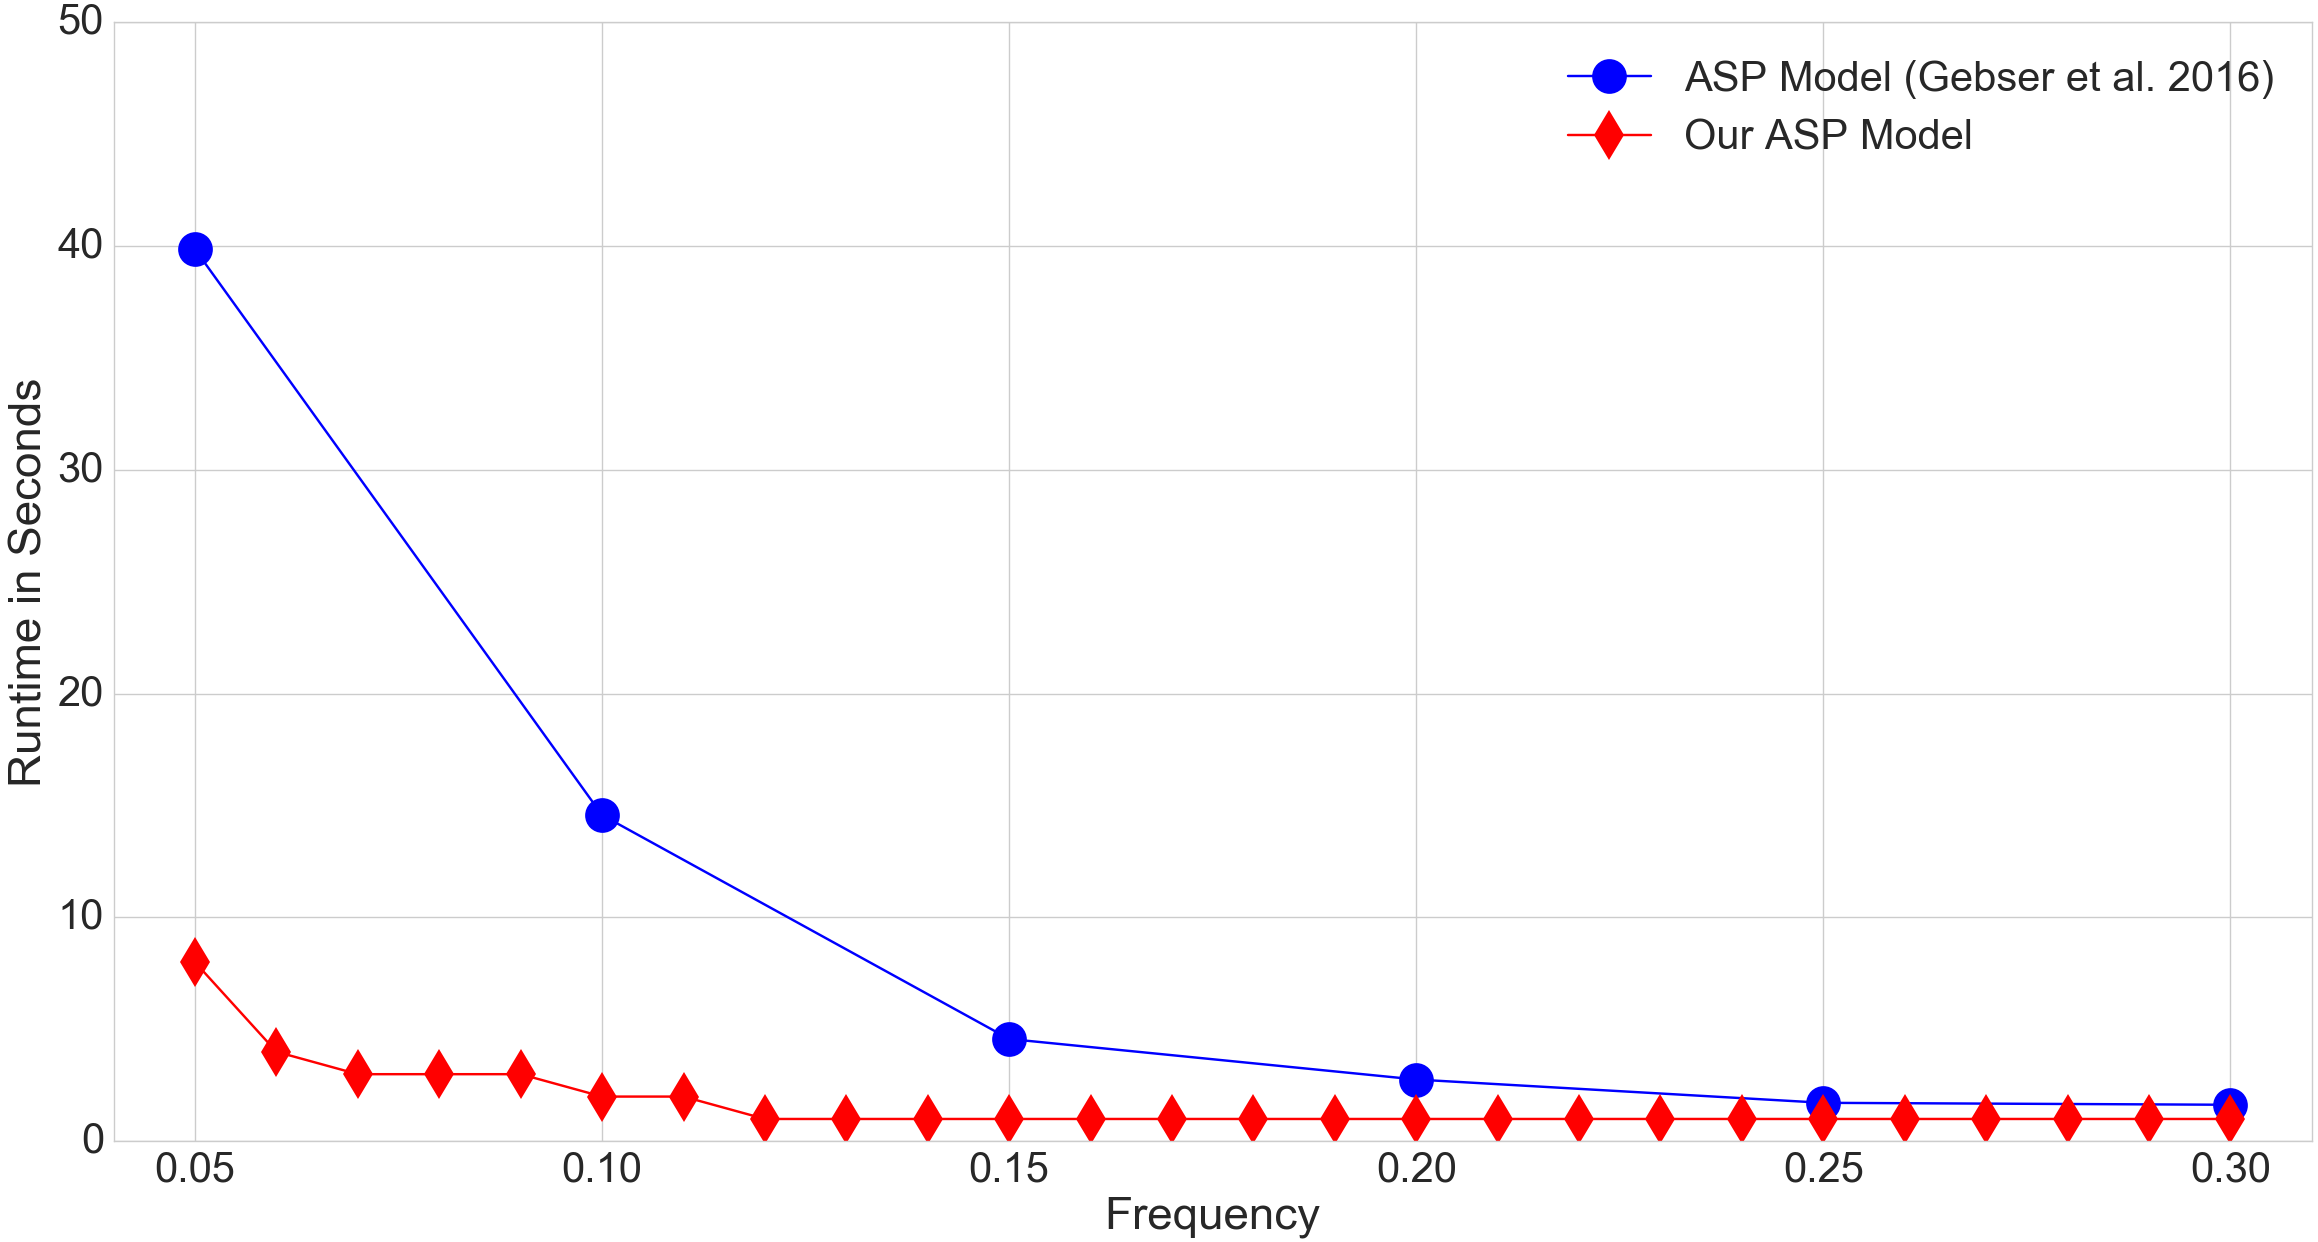
\includegraphics[width=\scalefigures\textwidth]{runtime_sequences_comparison.png}
   \caption{Comparing with ASP sequence model \parencite{DBLP:conf/ijcai/GebserGQ0S16} on the 200 generated sequences (closed)}
    \label{fig:sequence_comparison}
  \end{subfigure}
 \hfill
  \begin{subfigure}[t]{0.49\textwidth}
   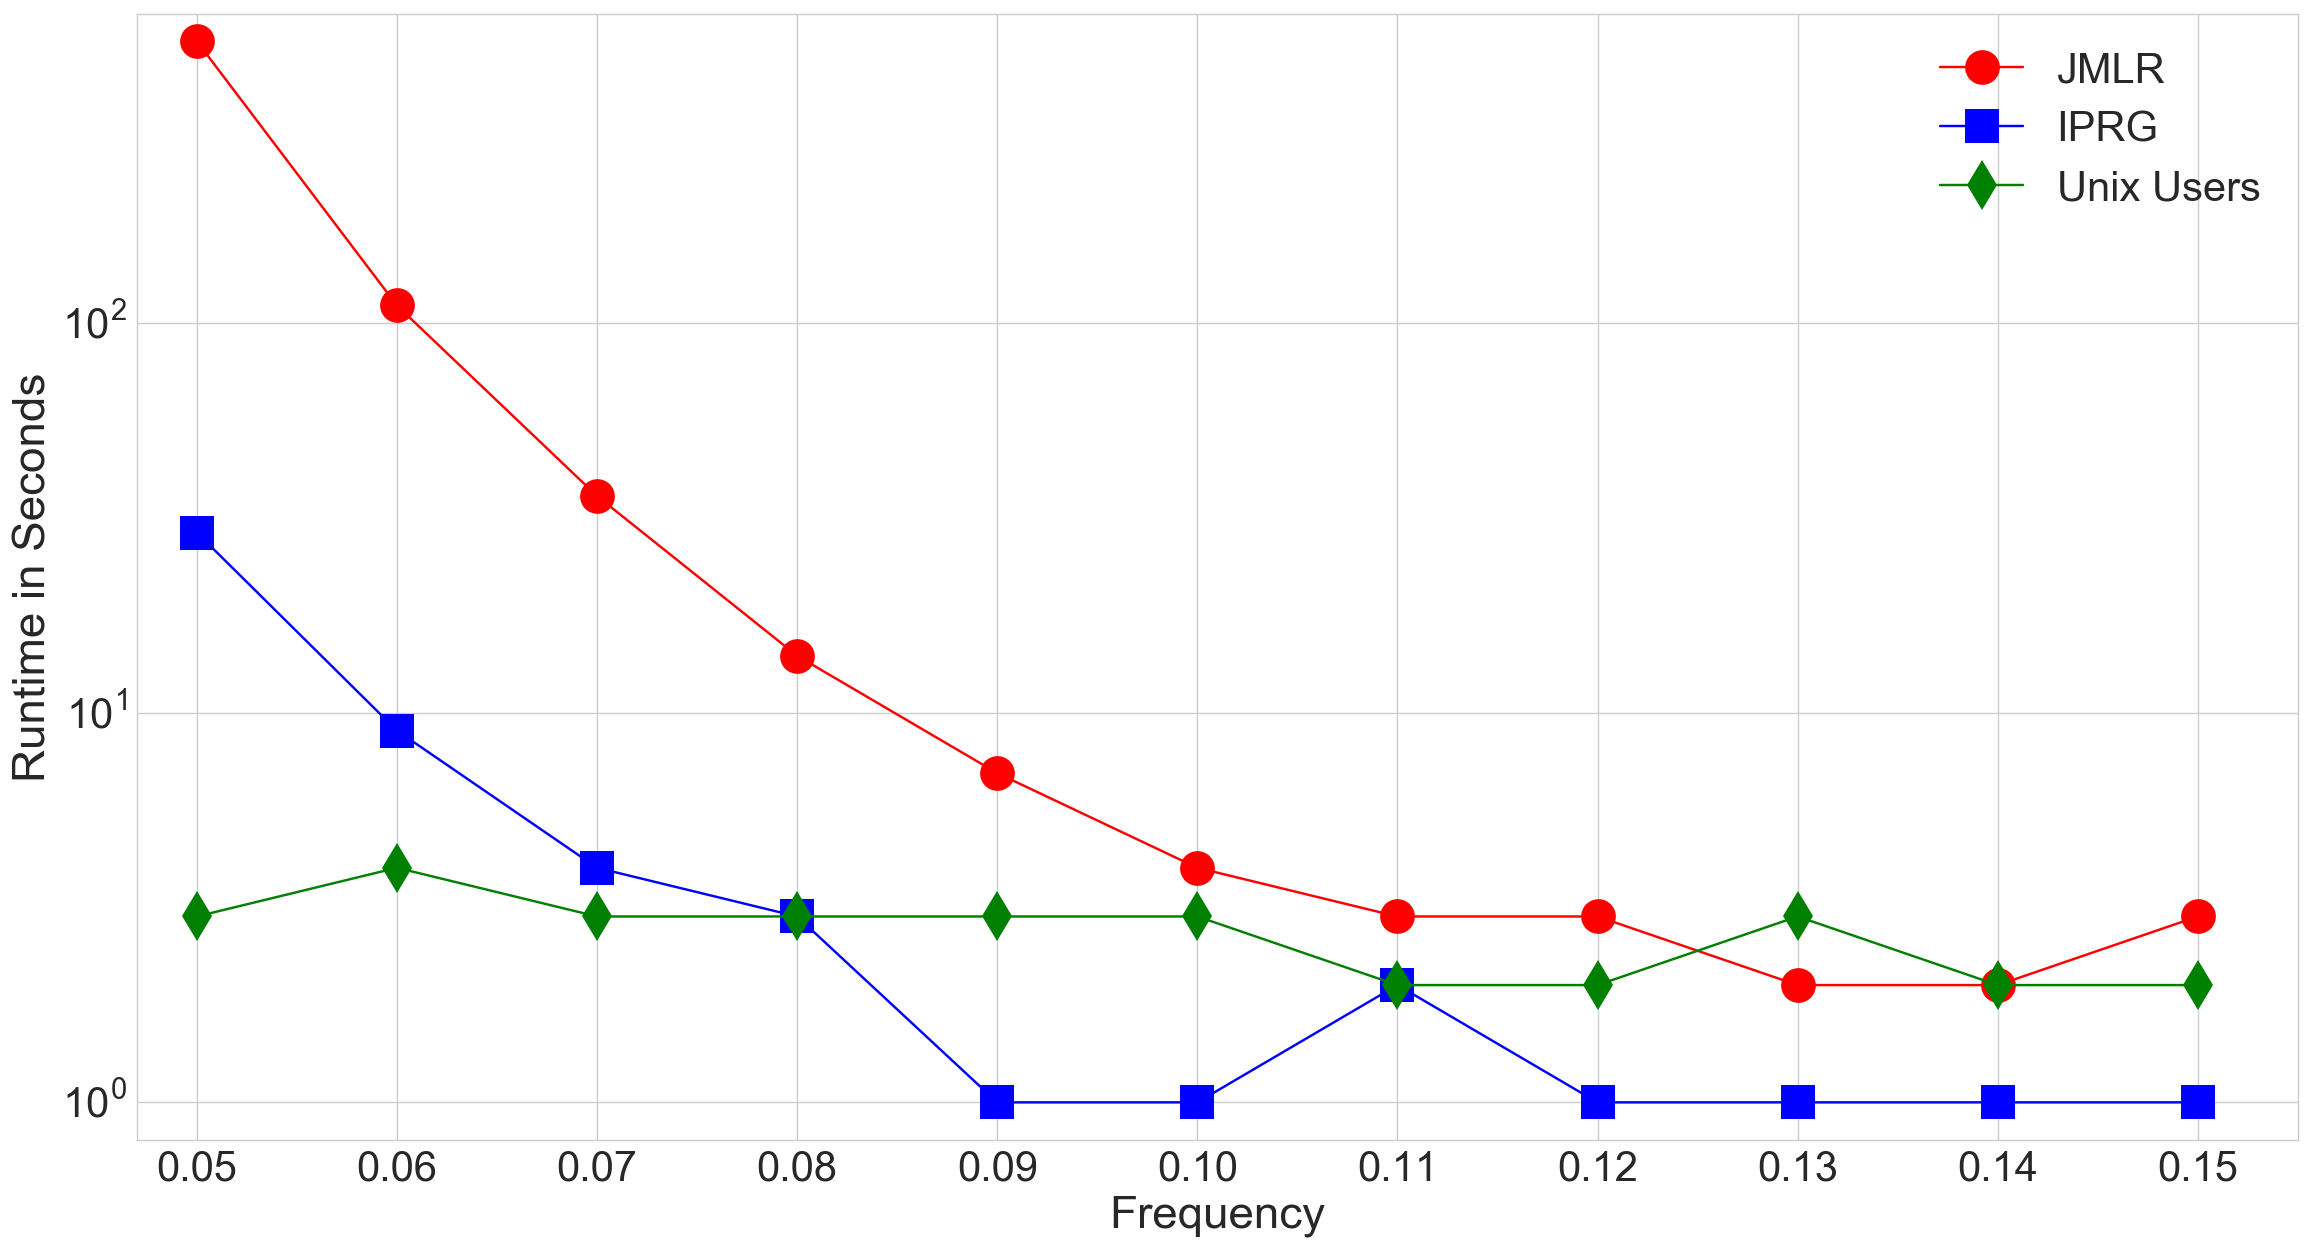
\includegraphics[width=\scalefigures\textwidth]{maximal.png}
   \caption{Maximal sequence patterns} %: JMLR, Unix Users and iPRG}
    \label{fig:maximal}
  \end{subfigure}
 \hfill
  \begin{subfigure}[t]{0.49\textwidth}
   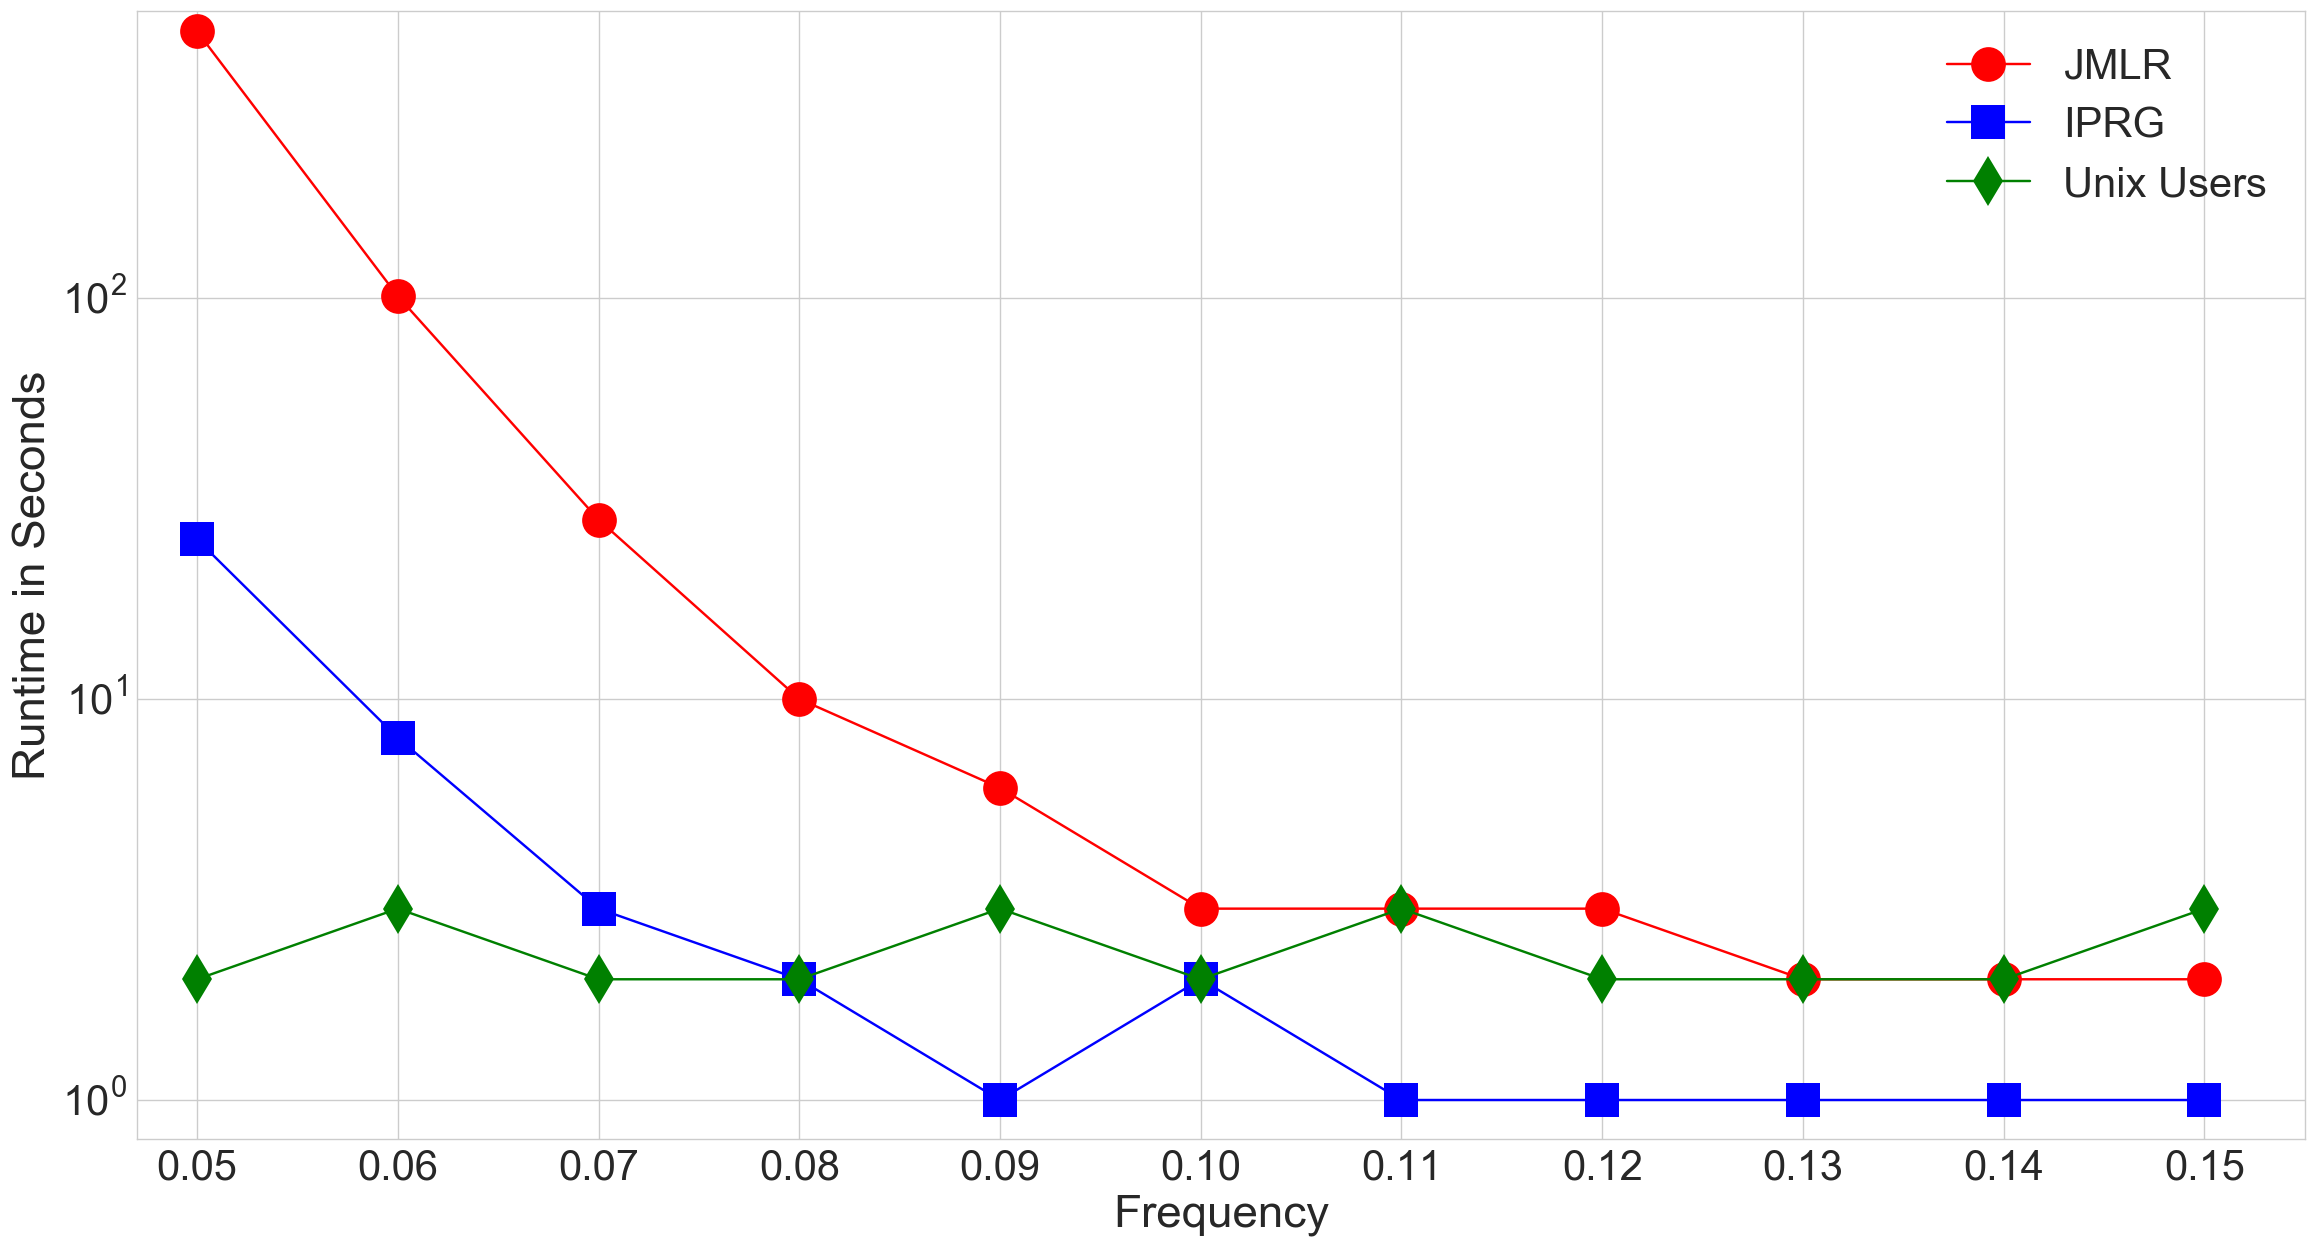
\includegraphics[width=\scalefigures\textwidth]{closed.png}
   \caption{Closed sequence patterns} %: JMLR, Unix Users and iPRG}
    \label{fig:closed}
  \end{subfigure}
\hfill
  \begin{subfigure}[t]{0.49\textwidth}
   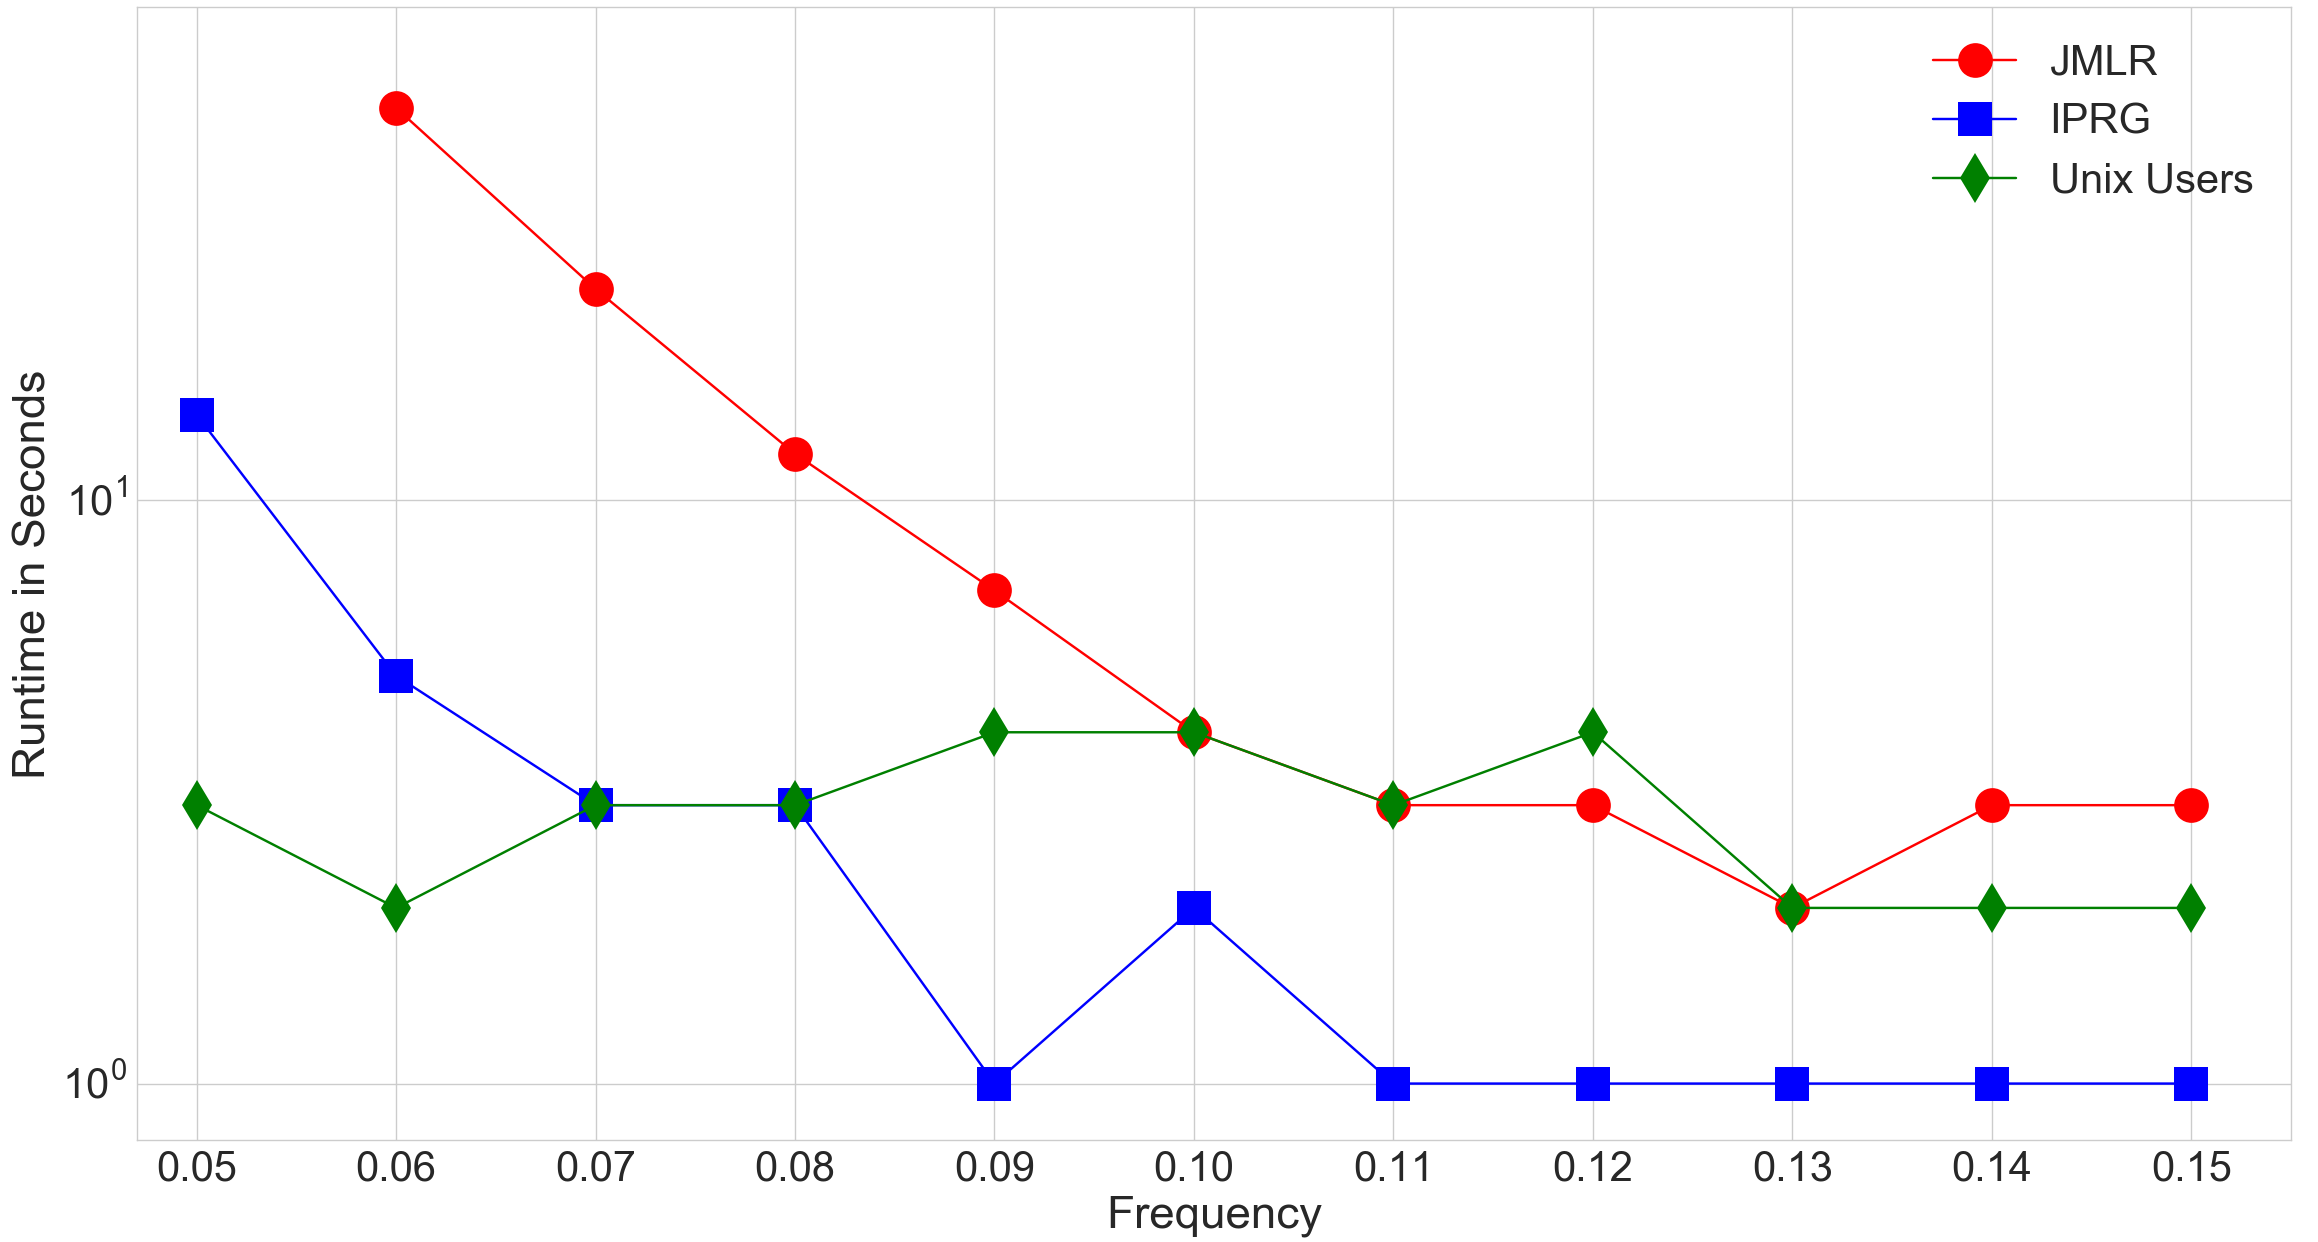
\includegraphics[width=\scalefigures\textwidth]{skyline.png}
   \caption{Skyline sequence patterns} %: JMLR, Unix Users and iPRG}
    \label{fig:skyline}
  \end{subfigure}
  \caption{Investigating \qone: comparison with pure ASP model (\ref{fig:sequence_comparison}) and maximal (\ref{fig:maximal}),  closed (\ref{fig:closed}), and skyline (\ref{fig:skyline}) sequence mining on  JMLR, Unix Users, and iPRG datasets.}
  \label{fig:qone}
\end{figure}

To investigate \qone, in Figure~\ref{fig:sequence_comparison}, we compare the ASP model \parencite{DBLP:conf/ijcai/GebserGQ0S16} with our method on the default 200 sequence sample, generated by the tool\footnote{\url{https://sites.google.com/site/aspseqmining}} of \textcite{DBLP:conf/ijcai/GebserGQ0S16}. We %have to 
performed the comparison on the synthetic data, as the sequence-mining model \parencite{DBLP:conf/ijcai/GebserGQ0S16} failed to compute condensed representations on any of the standard sequence datasets for any support threshold value within the timeout. One can observe that our method consistently outperforms the purely declarative approach of \textcite{DBLP:conf/ijcai/GebserGQ0S16} and the advantage naturally becomes more apparent for smaller frequency threshold values. %since within the time-limit of an hour the sequence-mining ASP model could not compute condensed representation on the datasets for any threshold value.
 
In Figs.~\ref{fig:maximal},~\ref{fig:closed} and~\ref{fig:skyline} (the point $0.05$ for JMLR is a timeout), we present the runtimes of our method for \emph{maximal, closed} and \emph{skyline} sequential pattern mining settings on JMRL, Unix Users and iPRG datasets. In contrast to \textcite{DBLP:conf/ijcai/GebserGQ0S16}, our method managed to produce results on all of these datasets for reasonable threshold values within a couple of minutes.
%(the runtime on Unix Users shows slight fluctuations within a couple of seconds). %\sergey{it is just runtime is low on that dataset, so 2 second fluctuations occur}). 
% The runtime of our method on datasets JMLR, Unix Users and iPRG %can be found 
% for \emph{closed}, \emph{maximal} and \emph{skyline} sequences are presented in Figure~\ref{fig:closed}, %\textit{maximal} in 
%  Figure~\ref{fig:maximal} and %\textit{skyline} in 
% Figure~\ref{fig:skyline} resp. Overall, we observe in Figure \ref{fig:qone} that our method provides better scalability and can be run within reasonable time on the real datasets, while covering the most popular condensed representation types as the model based only on ASP.

\begin{figure}[tb]
  \centering
  \begin{subfigure}[t]{0.49\textwidth}
   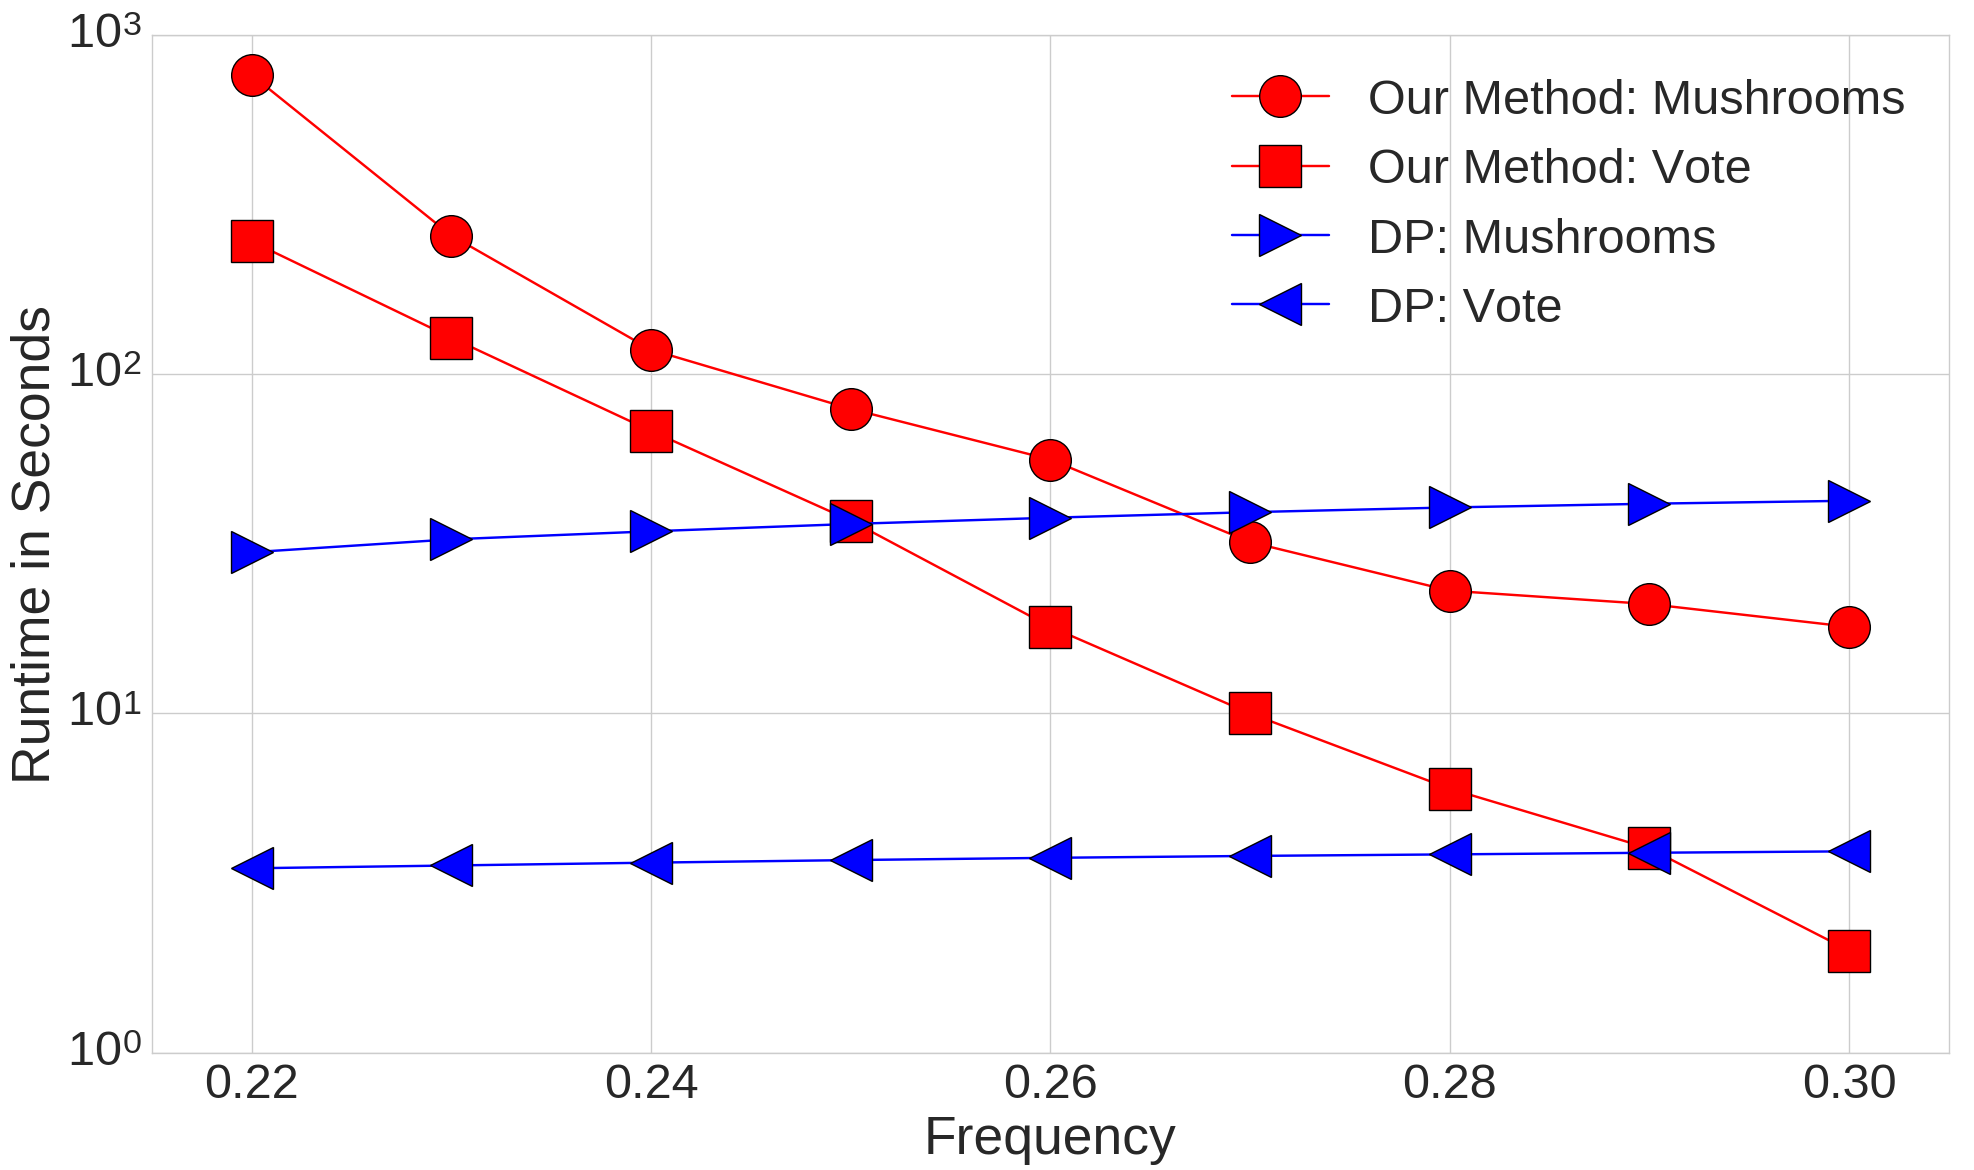
\includegraphics[width=\scalefigures\textwidth]{dp_maximal.png}
   \caption{Maximal itemset mining: comparing with DP on Vote and Mushrooms}
    \label{fig:dp_maximal}
  \end{subfigure}
 \hfill
  \begin{subfigure}[t]{0.49\textwidth}
   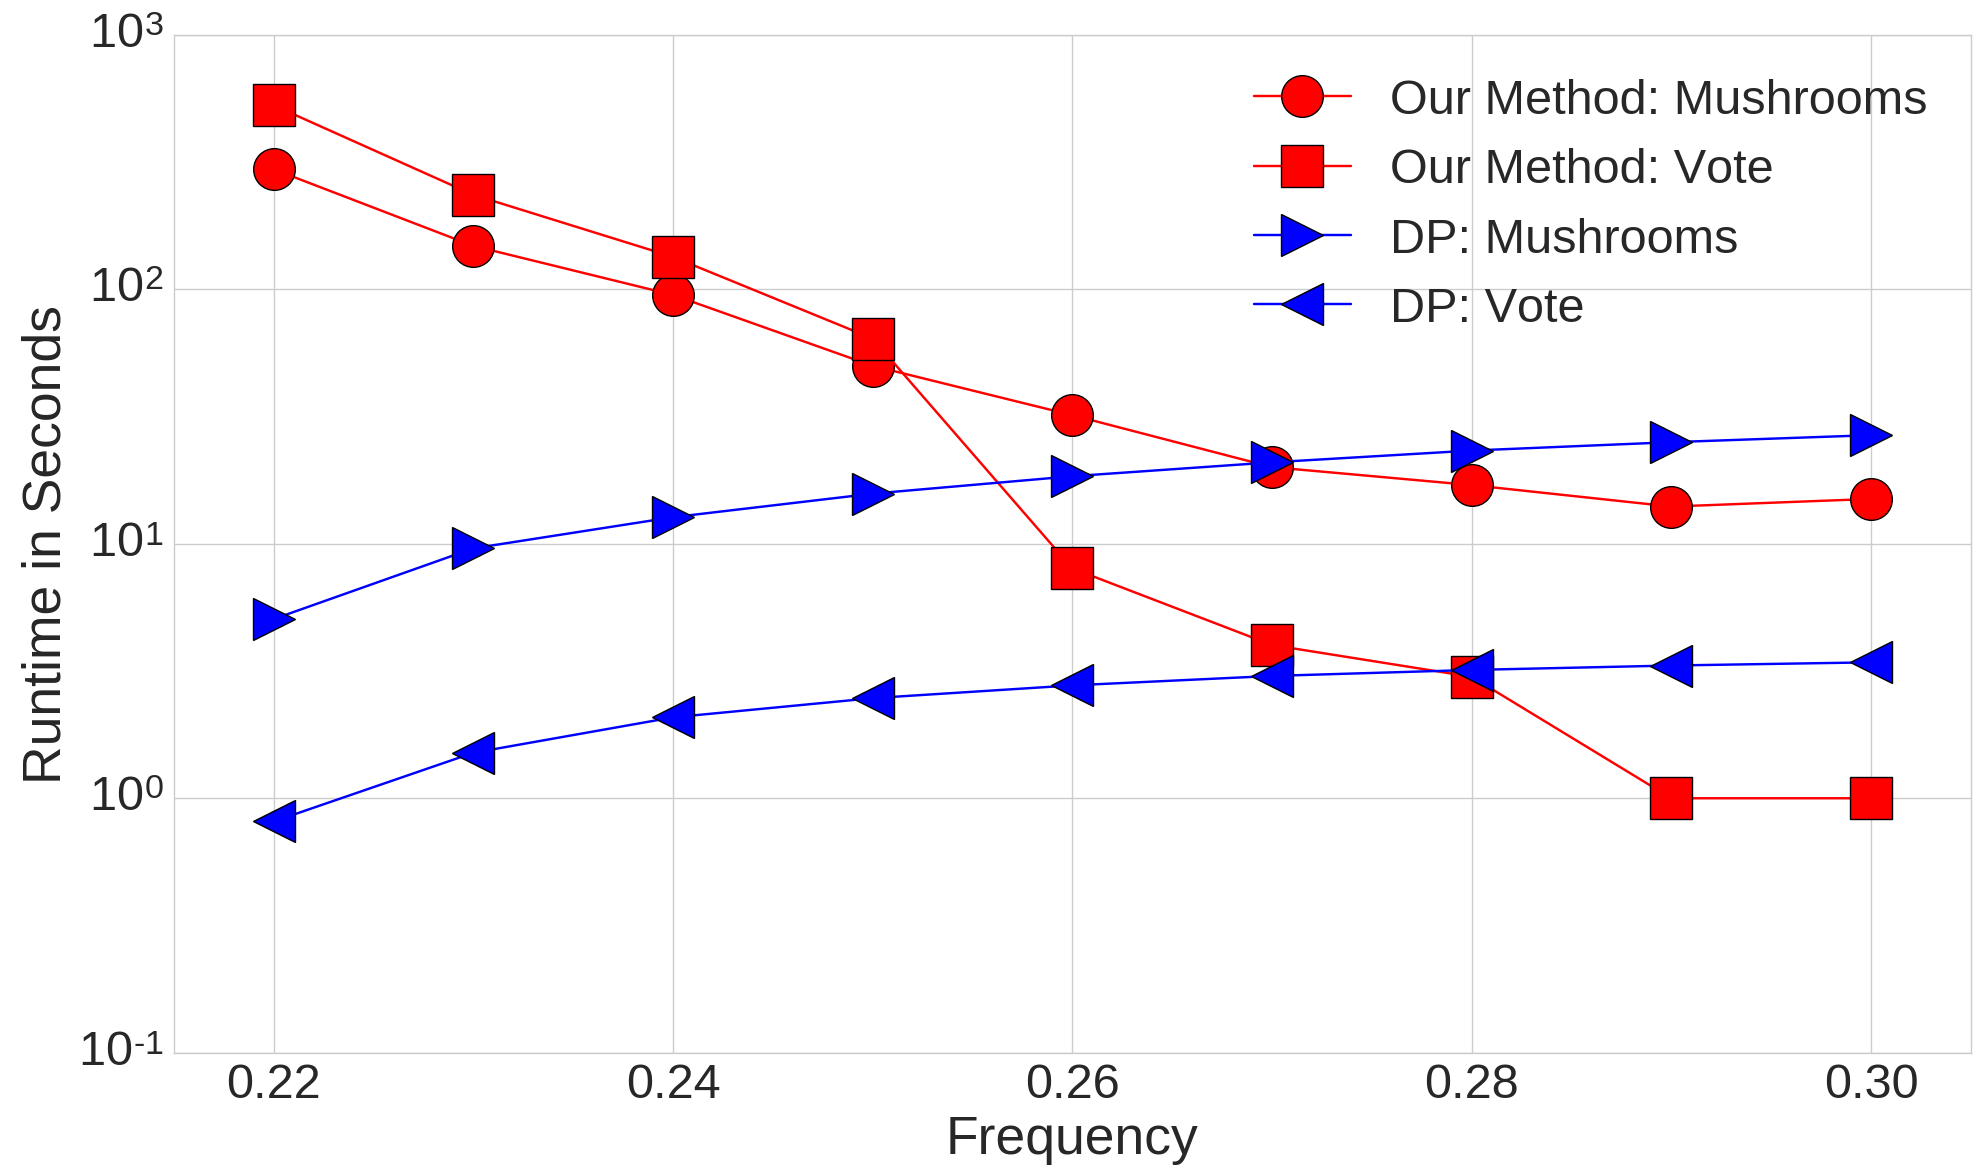
\includegraphics[width=\scalefigures\textwidth]{dp_closed}
   \caption{Closed itemset mining: comparing with DP on Vote and Mushrooms}
    \label{fig:dp_closed}
  \end{subfigure}
 \hfill
  \begin{subfigure}[t]{0.49\textwidth}
   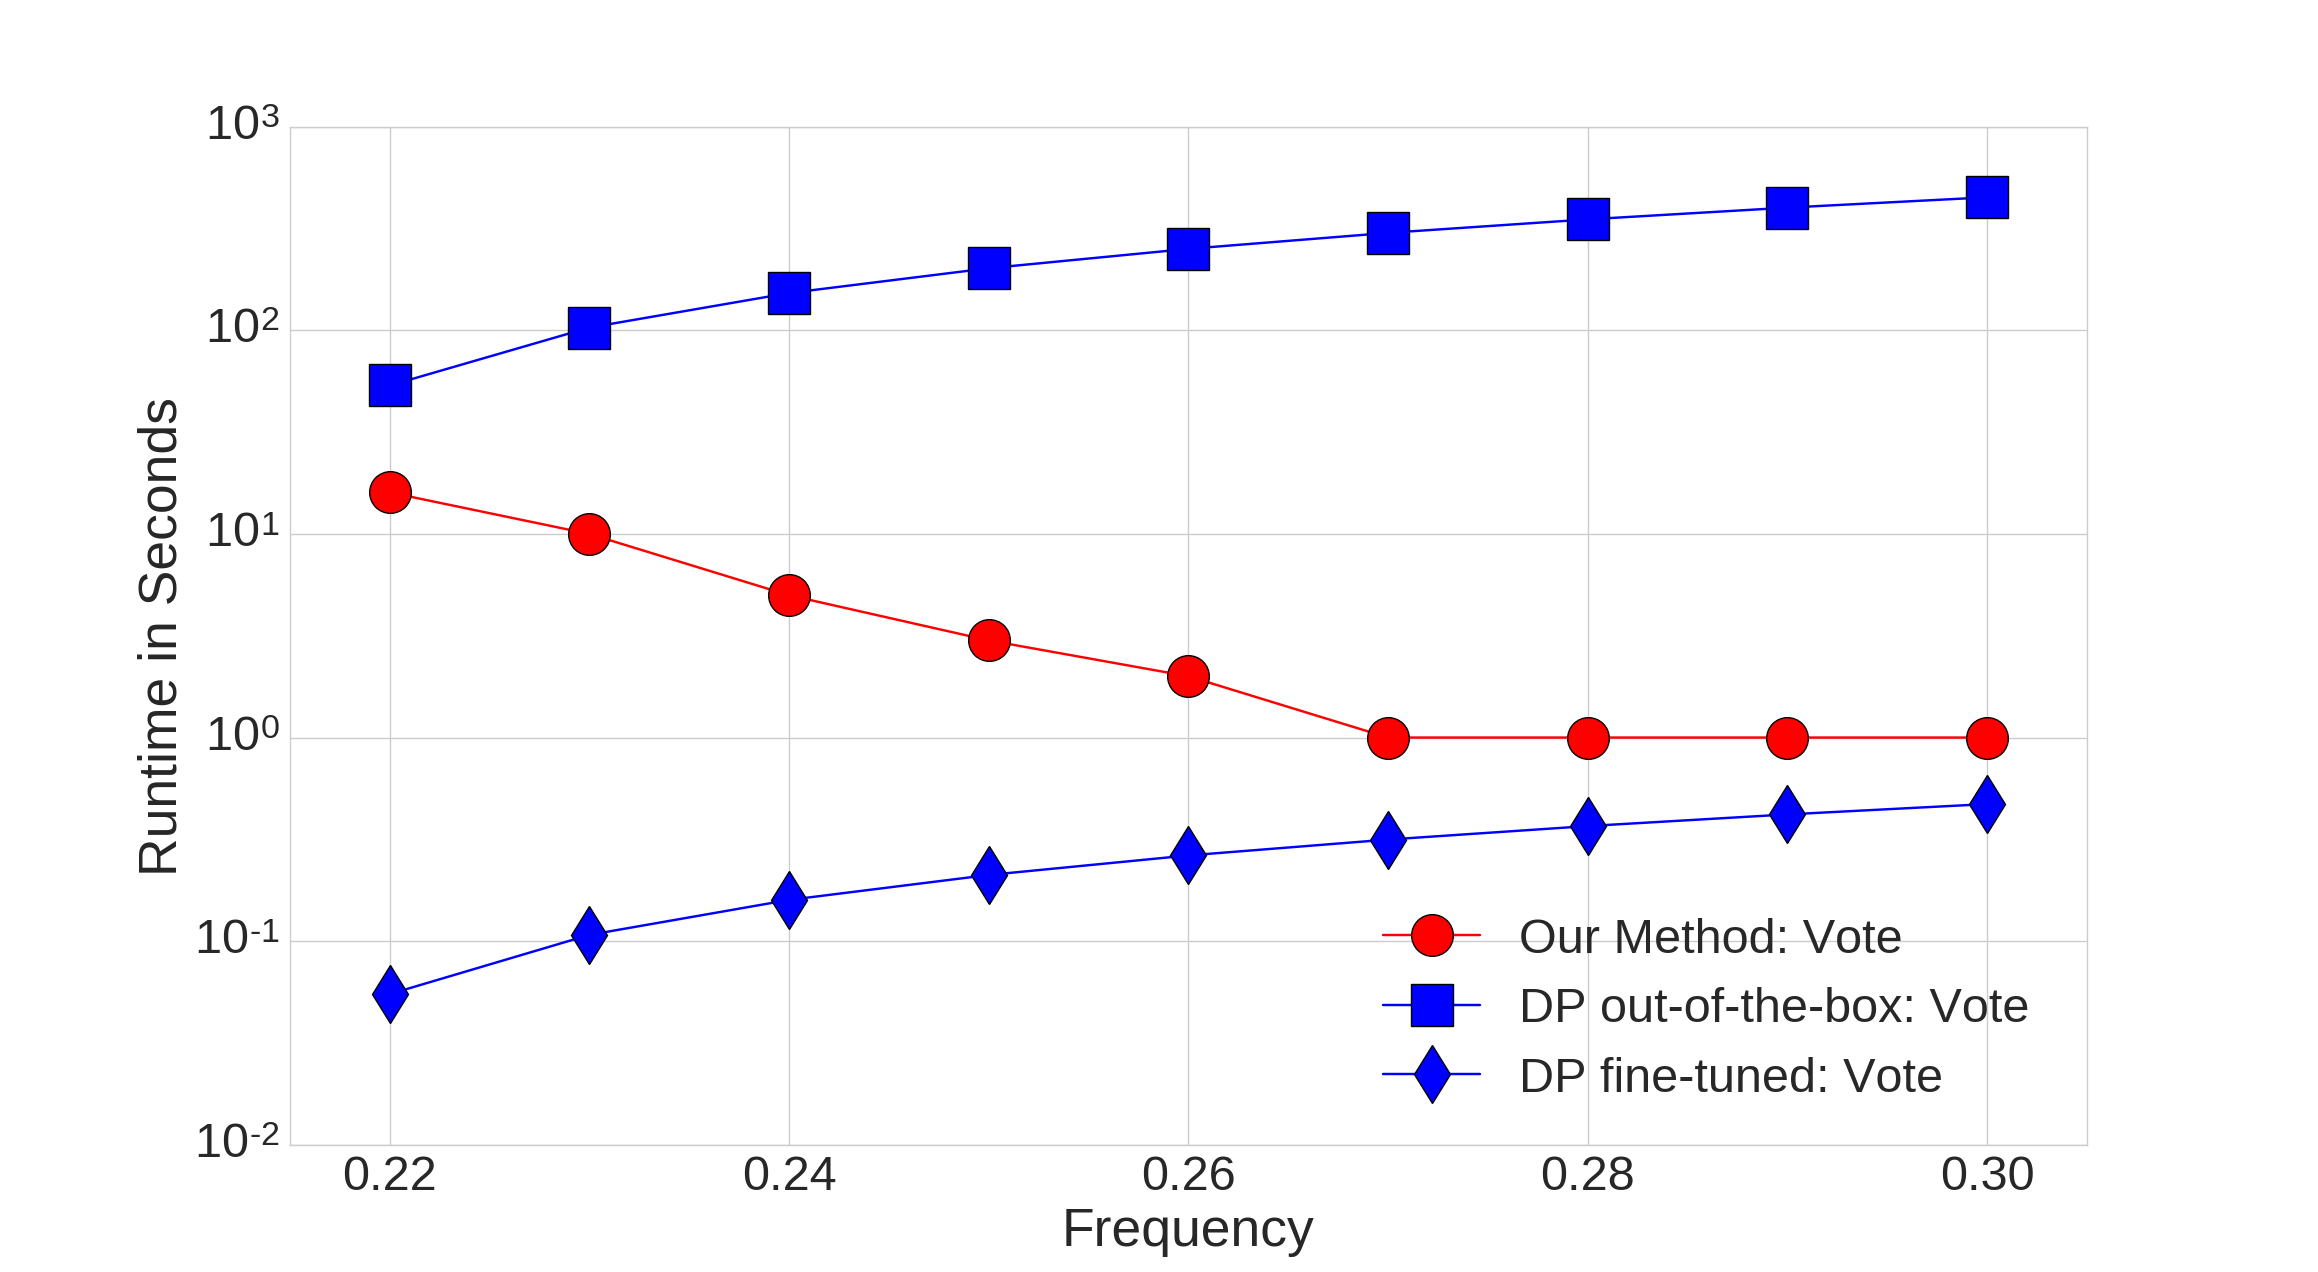
\includegraphics[width=\scalefigures\textwidth]{dp_skyline.png}
   \caption{Skyline itemset mining: comparing with out-of-the-box and fine-tuned DP on Vote}
    \label{fig:dp_skyline}
  \end{subfigure}
\hfill
  \begin{subfigure}[t]{0.49\textwidth}
   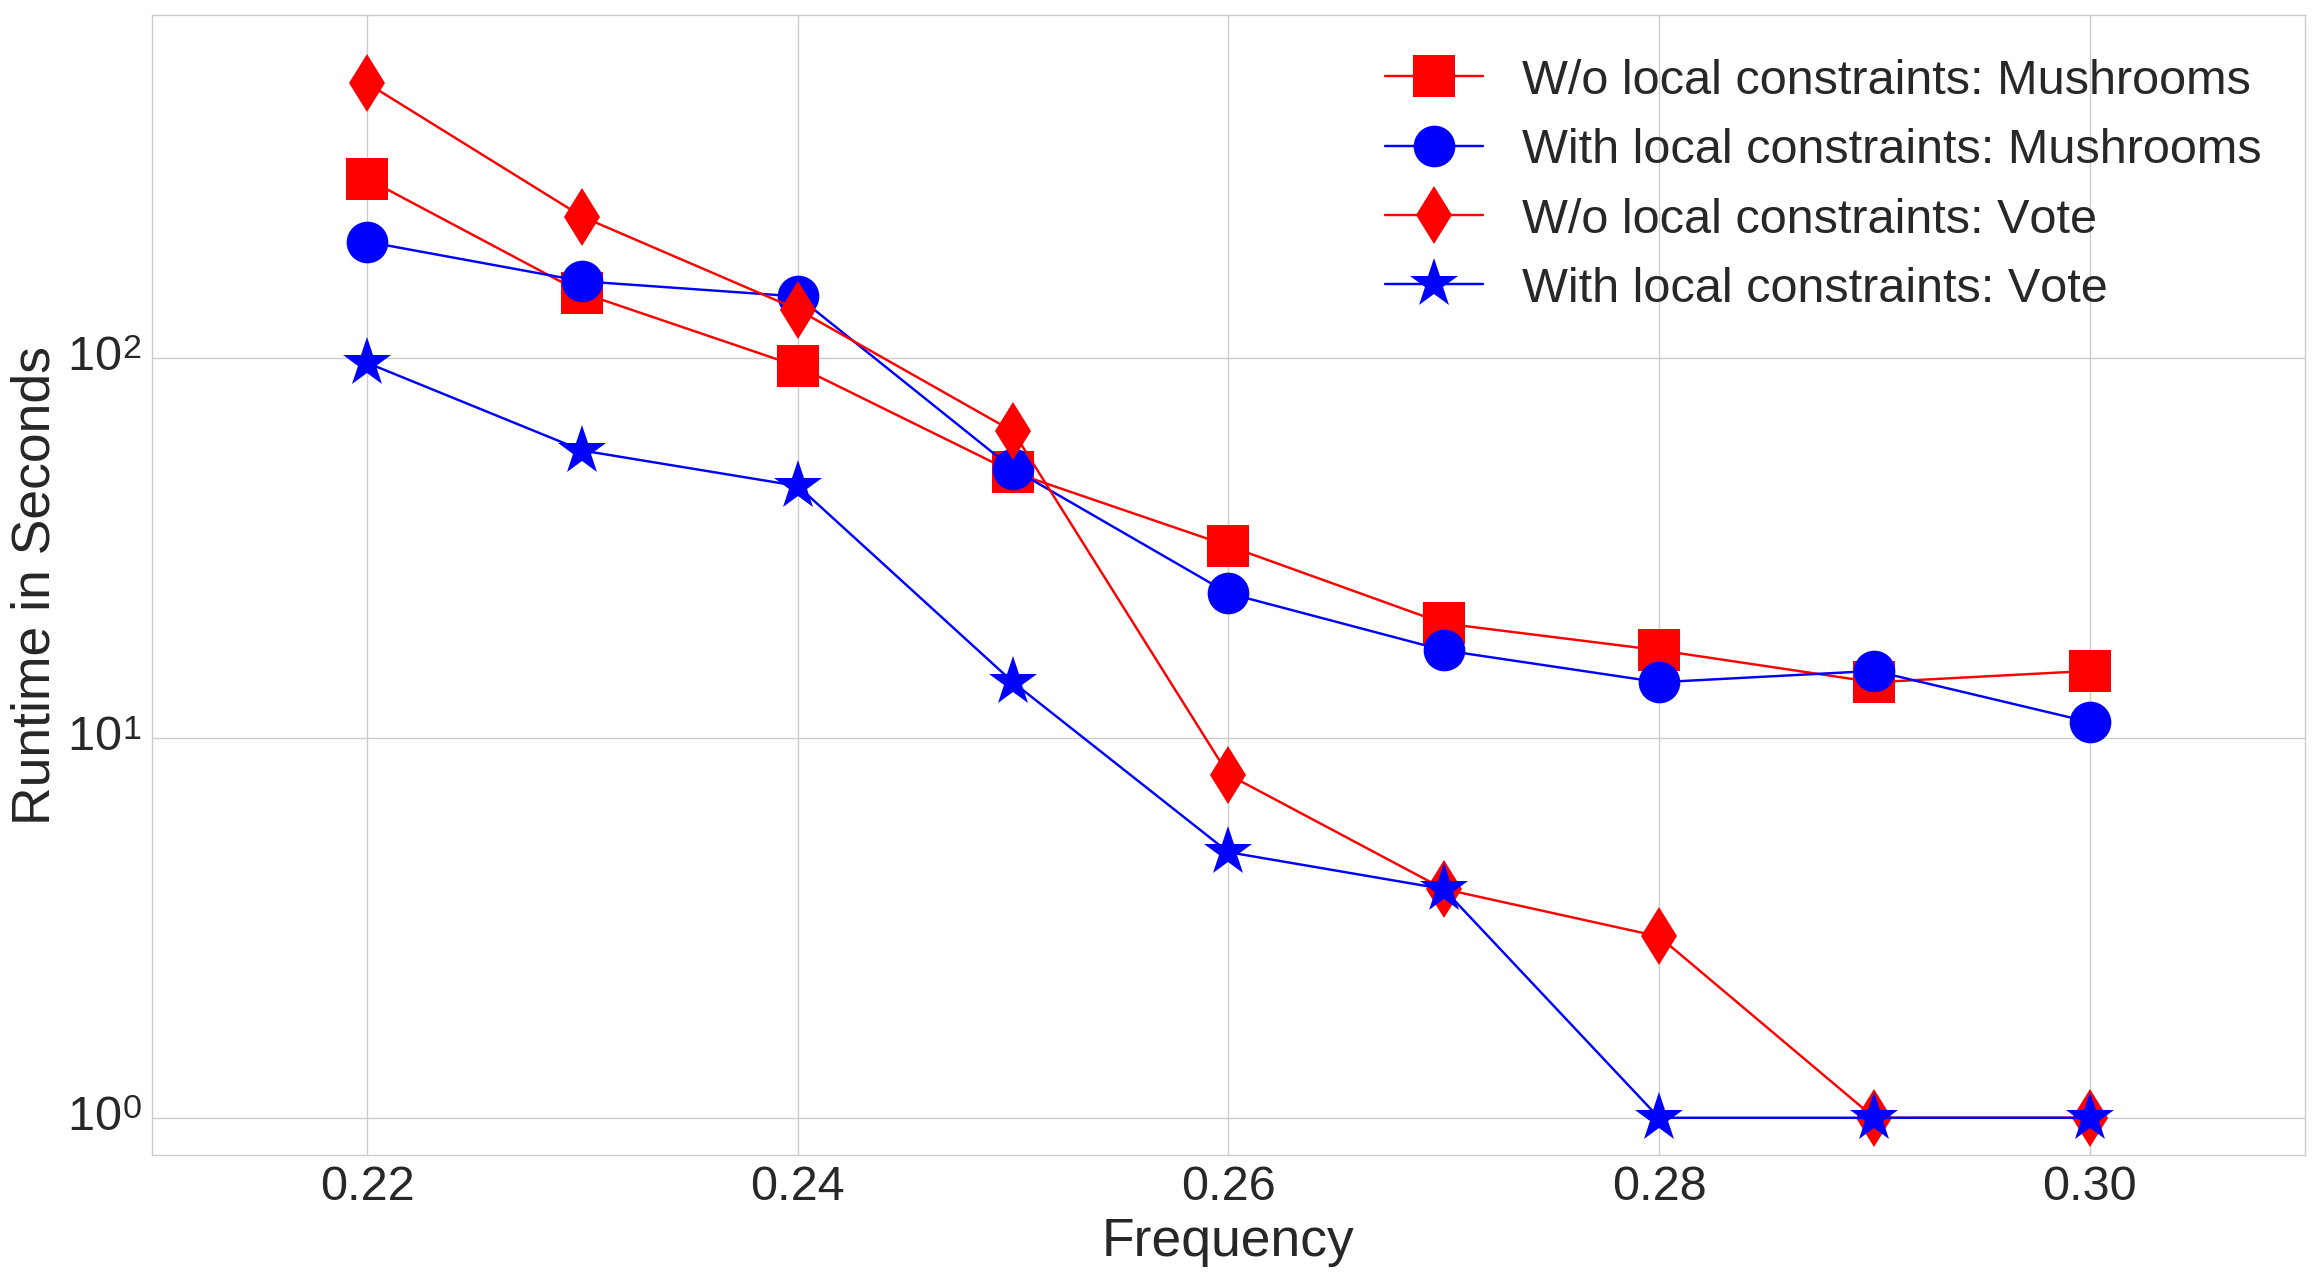
\includegraphics[width=\scalefigures\textwidth]{itemset_under_constraints.png}
   \caption{Closed itemset mining: our method with (w/o) local constraints on Vote and Mushrooms}%: local constraint enable faster propagation and speedup the search}
    \label{fig:local_constraints}
  \end{subfigure}
  % \caption{Investigating \qtwo: comparison with DP \parencite{dp2013} (\ref{fig:dp_closed}, \ref{fig:dp_maximal}, \ref{fig:dp_skyline}); and \qthree: the effect of local constraints on runtime (\ref{fig:local_constraints})}
  \label{fig:qtwo_three}
\end{figure}


To investigate \qtwo, we compare out-of-the-box performance of DP \parencite{dp2013} with our approach on maximal, closed and skyline itemset mining problems using standard datasets Vote and Mushrooms. As we see in Figs.~\ref{fig:dp_maximal} and \ref{fig:dp_closed}, on average, DP is one-to-two orders of magnitude faster; this gap is, however, diminishing as the minimum frequency increases. %as the frequency grows. 
%What is more surprising, 
Surprisingly, our approach is significantly faster than DP out-of-the-box for skyline patterns (Figure~\ref{fig:dp_skyline}); this holds also for the Mushrooms dataset, not presented here. 

Fine-tuning parameters of DP by changing the order in which operators are applied within the system (skyline+ option) allowed to close this gap. With this adaptation DP demonstrates one-to-two orders of magnitude better performance, as can be seen in Figure~\ref{fig:dp_skyline}. However, fine-tuning such a system requires the understanding of its inner mechanisms or exhaustive application of all available options. 
% It is possible to fine-tune DP to change its behavior to close this gap. More specifically, we analyzed all options of DP and found that besides the default flag \textit{skyline} for skyline patterns, the option \textit{skyline+} is also available, which computes the same patterns but applies operators in a different order. Then DP 

To %investigate 
address \qthree we introduced three simple local constraints %into 
for the itemset mining setting from \qtwo: %. Namely, we used 
two size constraints $\textit{size(I)} > 2$ and $\textit{size(I)} < 7$ and a cost constraint: each item gets weight equal to its value with the maximal budget of $n$, which is set to $20$ in the experiments. % (Vote has 435 transactions and 48 binary items and Mushrooms has 8124 and 119 resp.). 

In Figure~\ref{fig:local_constraints}, we present the results for closed itemset mining with and without local constraints (%other 
experiments with other global constraints demonstrate a similar runtime pattern). % and are not depicted here for space reasons).
%\comment{PM: Can we cite space reasons in a journal paper? Maybe just drop everything after and including ``and are not''.}
% One can see that 
Local constraints ensure %allow for 
better propagation and speed up the search. One of the key design features of our encoding is the filtering technique used to select candidate patterns among only valid patterns. Its effect can be clearly seen, e.g., for the Vote dataset in Figure~\ref{fig:local_constraints}, where for certain frequencies the runtime gap is close to an order of magnitude.

\begin{figure}[tb]
  \centering
  \begin{subfigure}[t]{0.49\textwidth}
   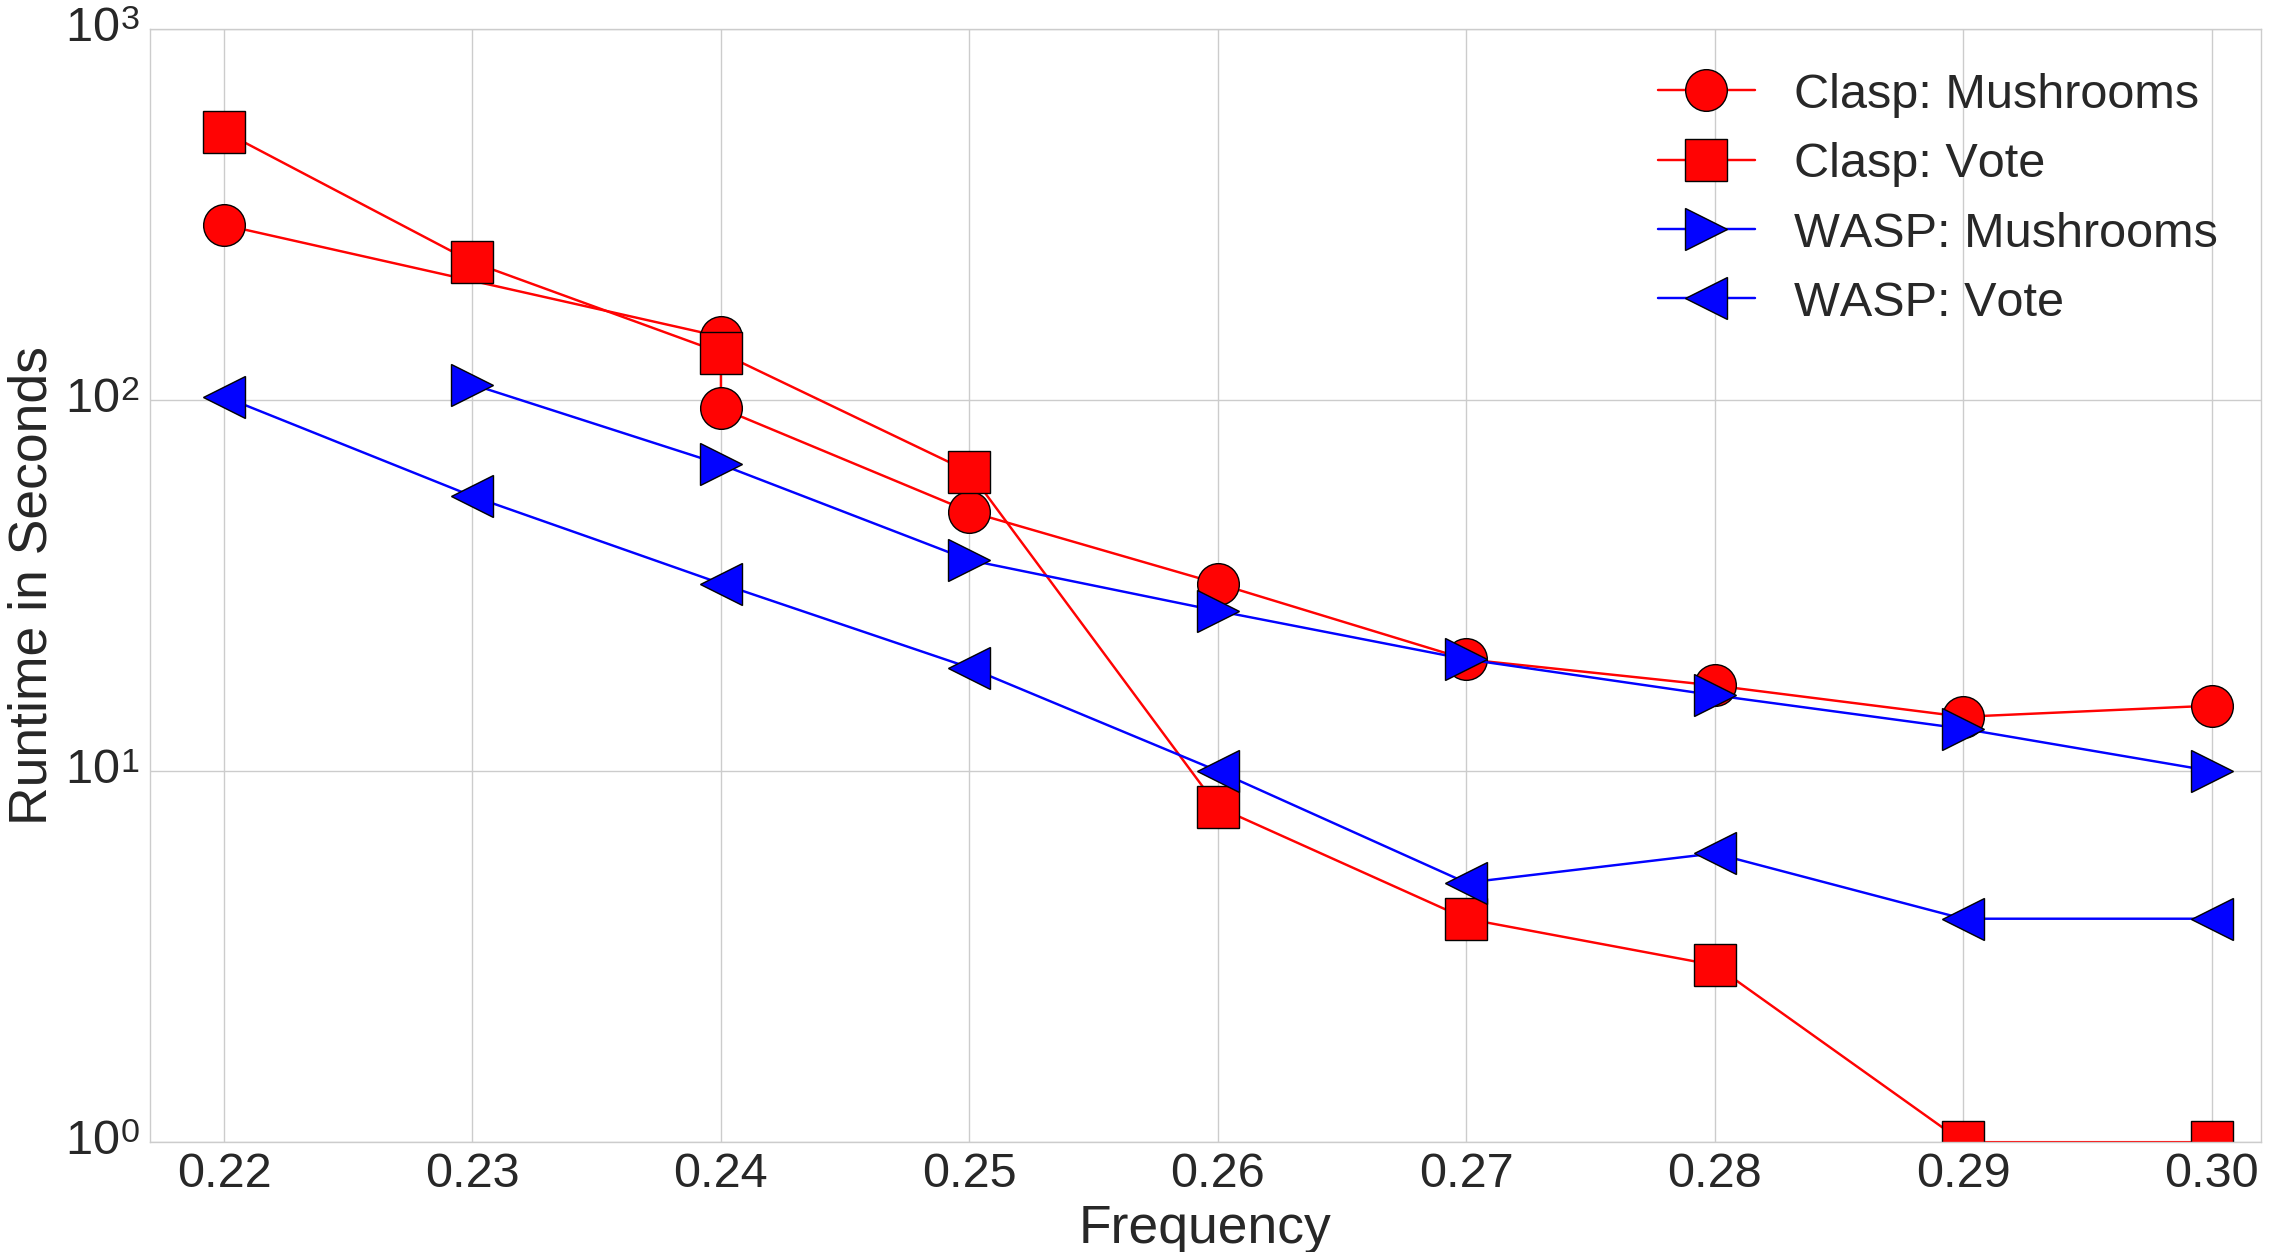
\includegraphics[width=\scalefigures\textwidth]{closed_WASP_vs_Clasp.png}
   \caption{Itemset mining: closed patterns}
    \label{fig:itemset_wasp_closed_comparison}
  \end{subfigure}
 \hfill
  \begin{subfigure}[t]{0.49\textwidth}
   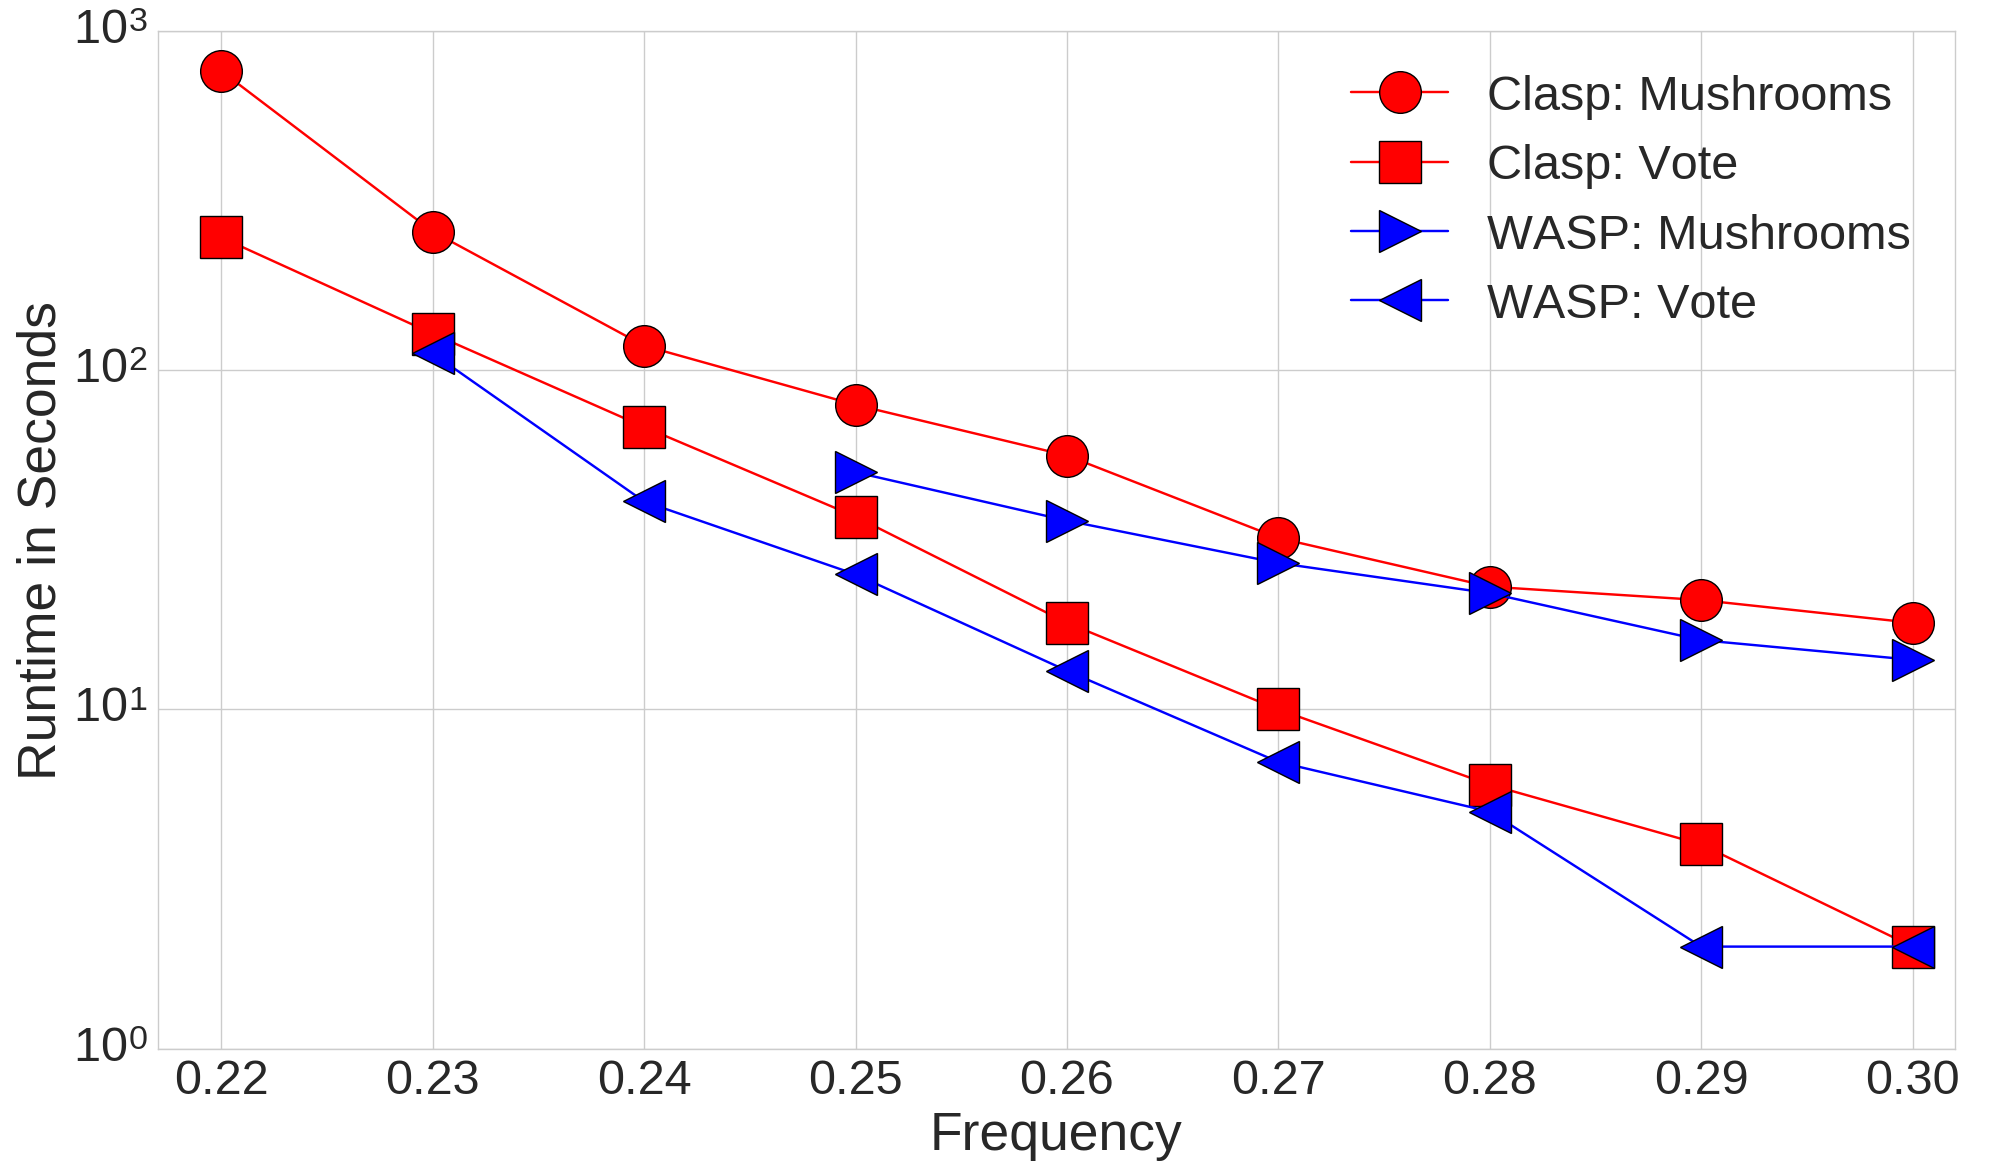
\includegraphics[width=\scalefigures\textwidth]{maximal_WASP_vs_Clasp.png}
   \caption{Itemset mining: maximal patterns} 
   \label{fig:itemset_wasp_max_comparison}
  \end{subfigure}
 \hfill
  \begin{subfigure}[t]{0.49\textwidth}
   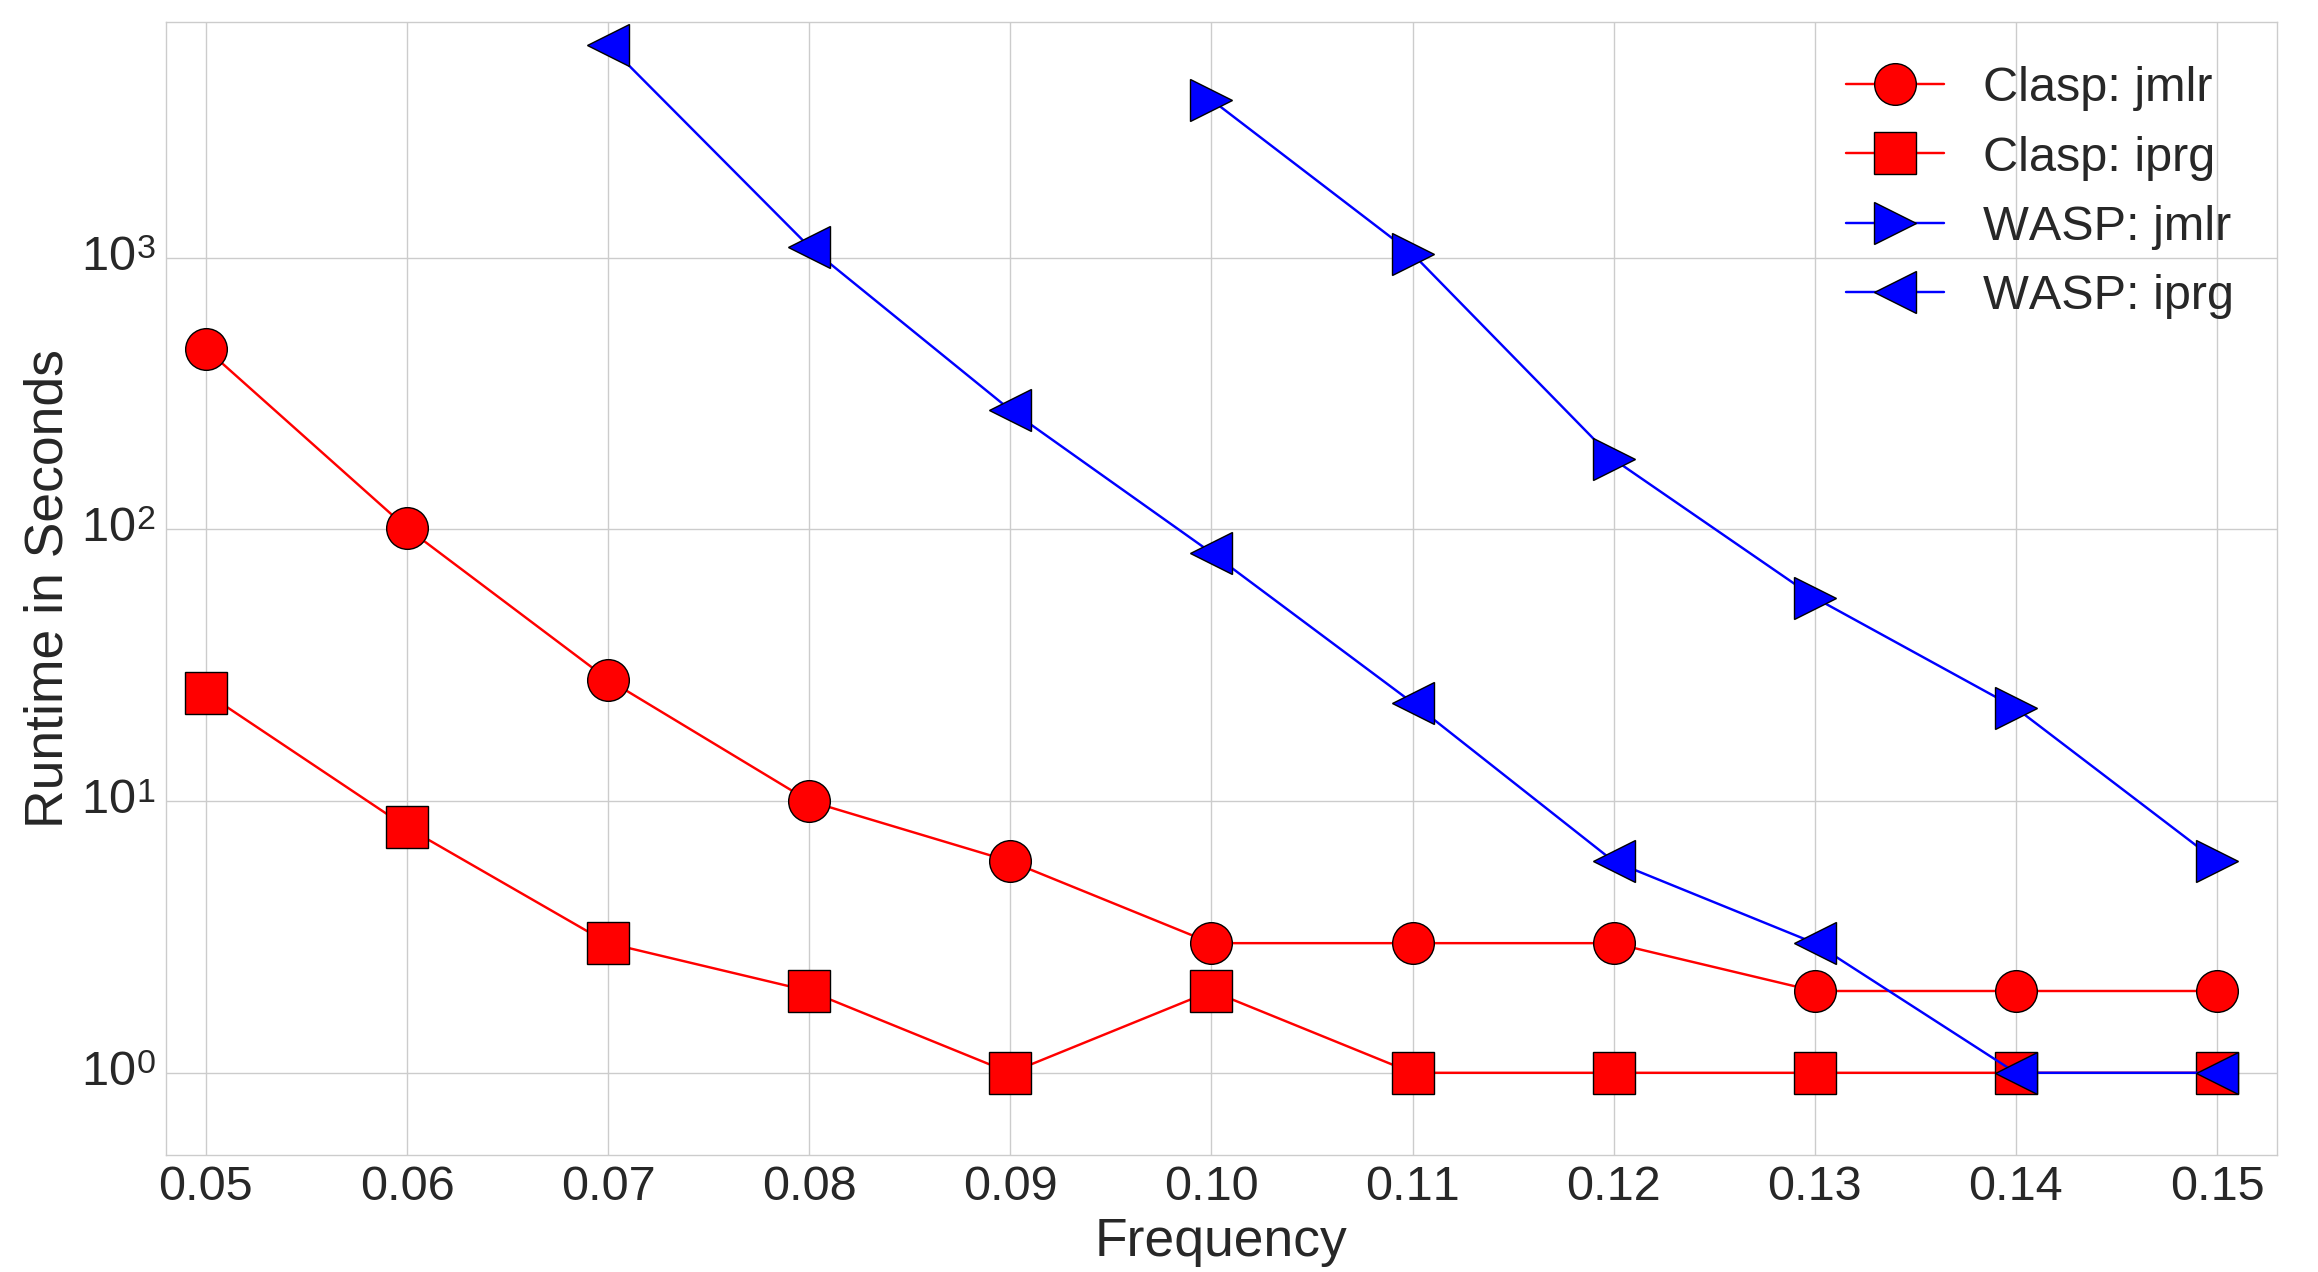
\includegraphics[width=\scalefigures\textwidth]{sequences_wasp_clasp_closed.png}
	\caption{Sequence mining: closed patterns}
	\label{fig:seq_wasp_closed_comparison}
  \end{subfigure}
\hfill
  \begin{subfigure}[t]{0.49\textwidth}
   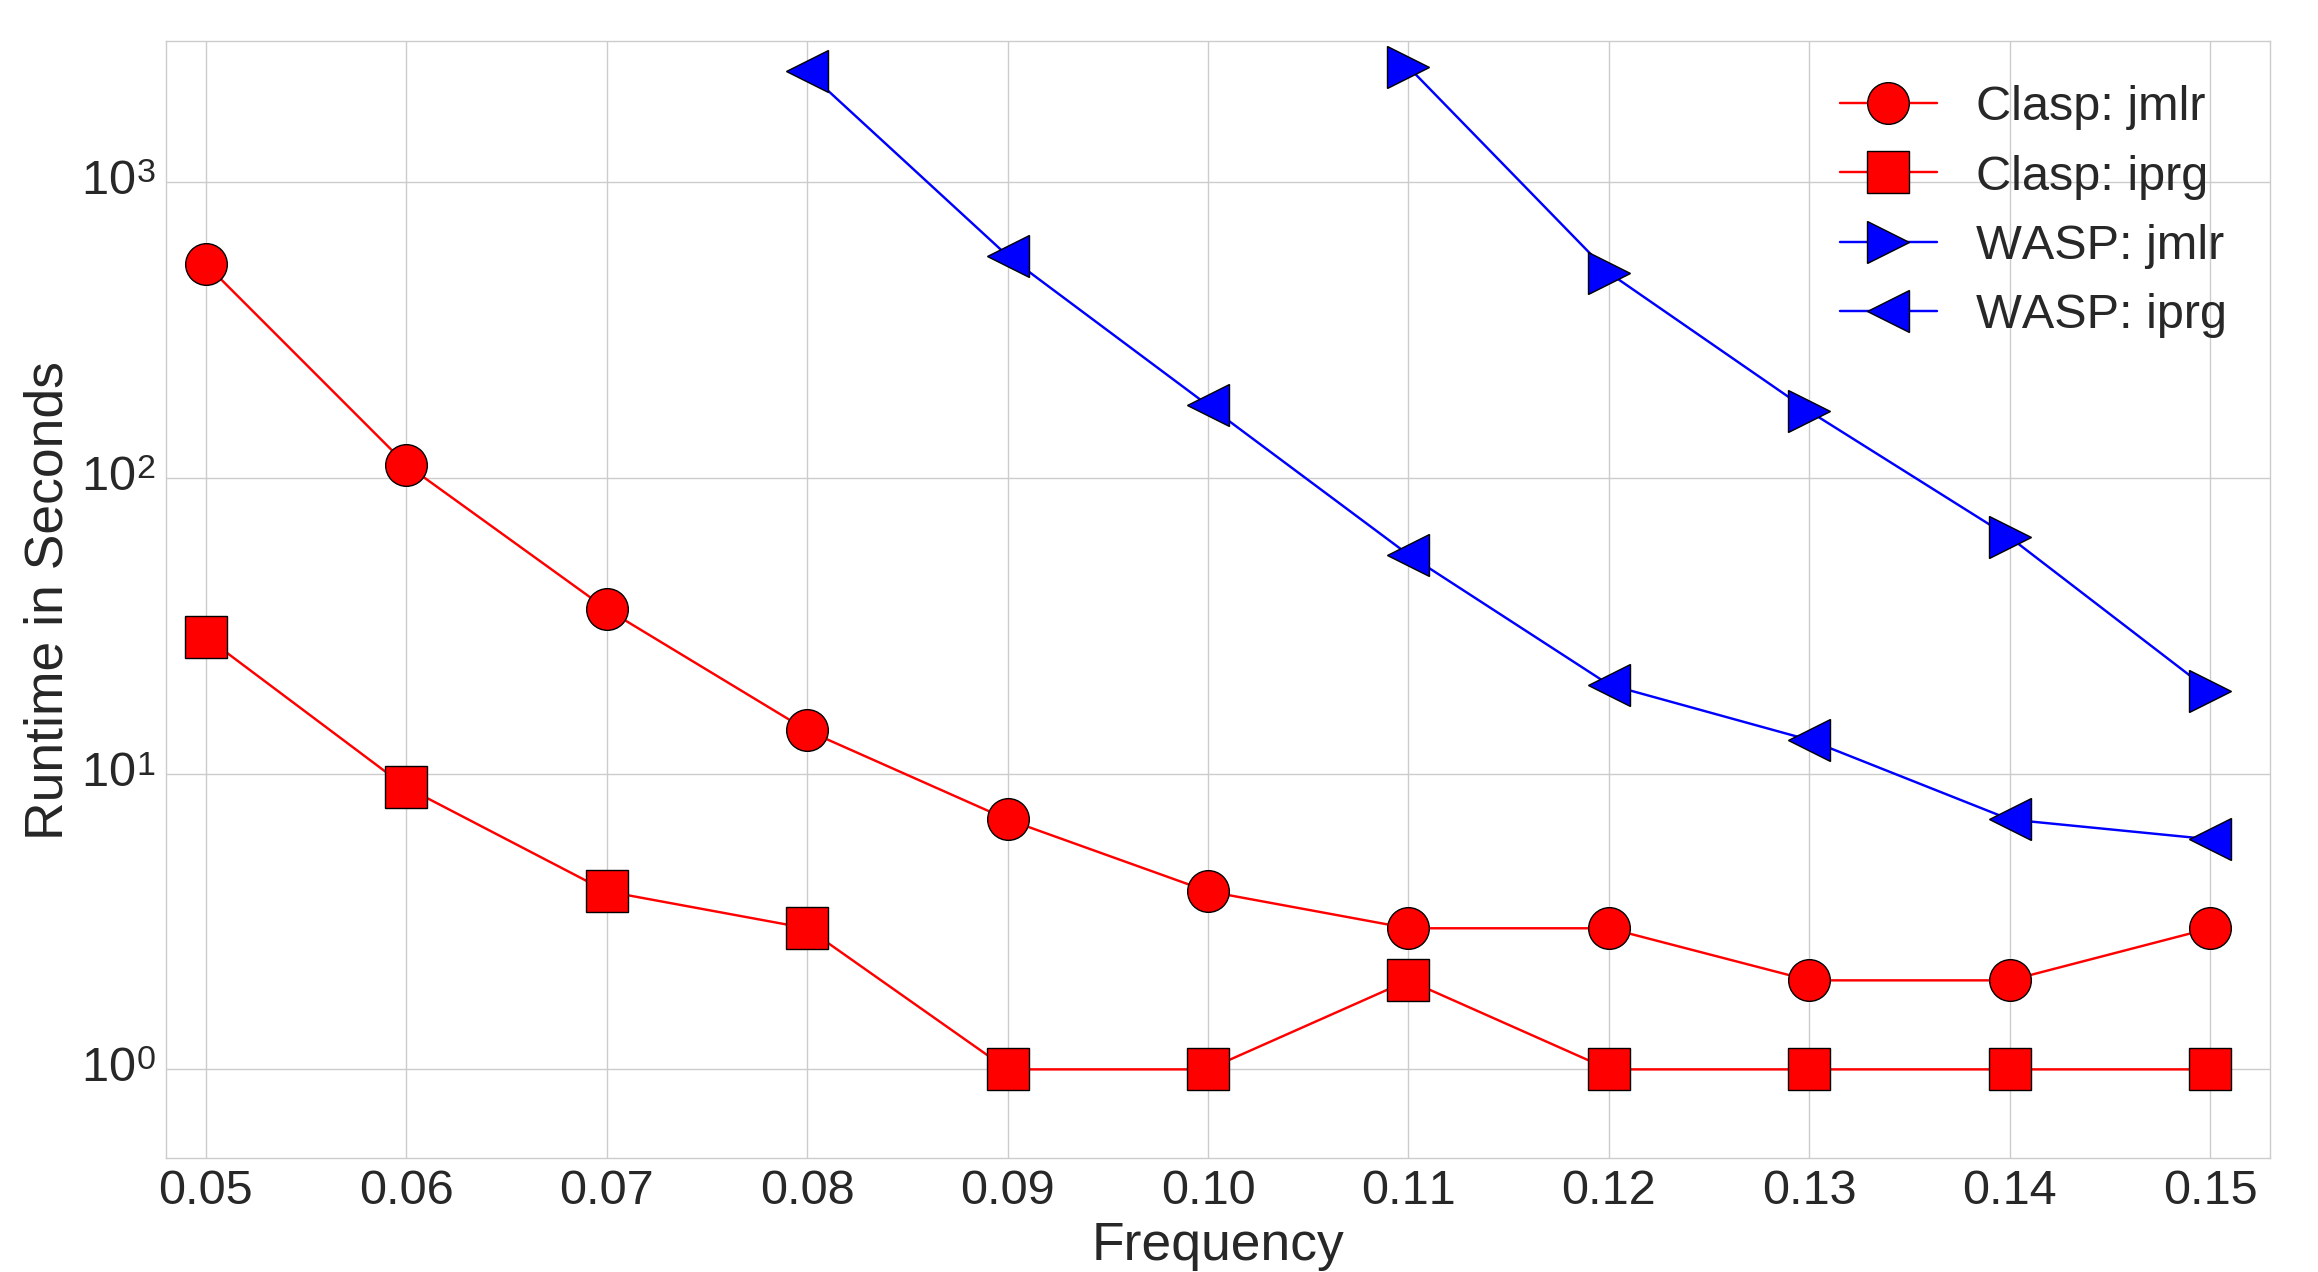
\includegraphics[width=\scalefigures\textwidth]{seq_clasp_wasp_max.png}
   \caption{Sequence mining: maximal patterns}
    \label{fig:seq_wasp_max_comparison}
  \end{subfigure}
    \label{fig:wasp_comparison}
	\caption{\qfour: comparing ASP solvers performance -- WASP and Clasp on itemset and sequence mining tasks}
\end{figure}


To analyze \qfour, we have replaced Clasp solver with WASP \parencite{wasp} in our system. As we see in Figure~\ref{fig:itemset_wasp_closed_comparison}, for mining closed itemsets two systems perform on par except for a timeout of WASP on mushrooms with frequency 0.22. However, we already can observe significant difference in performance on maximal patterns for both itemsets and sequences. A similar behavior can be seen in the setting of closed sequences mining: there is at least an order of magnitude difference in performance. The runtime gap cannot be explained by differences in grounding, since for both tasks Gringo has been used. However, we have noticed the difference in memory management: Clasp seems to be able to reason and keep track of significantly larger sets of patterns, while being economic and provident with memory. Since the task naturally allows one to generate problem instances of practically any size, we presume that our setting might be well-suited as one of the tests for ASP solvers' performance.

\begin{figure}[tb]
  \centering
  \begin{subfigure}[t]{0.49\textwidth}
   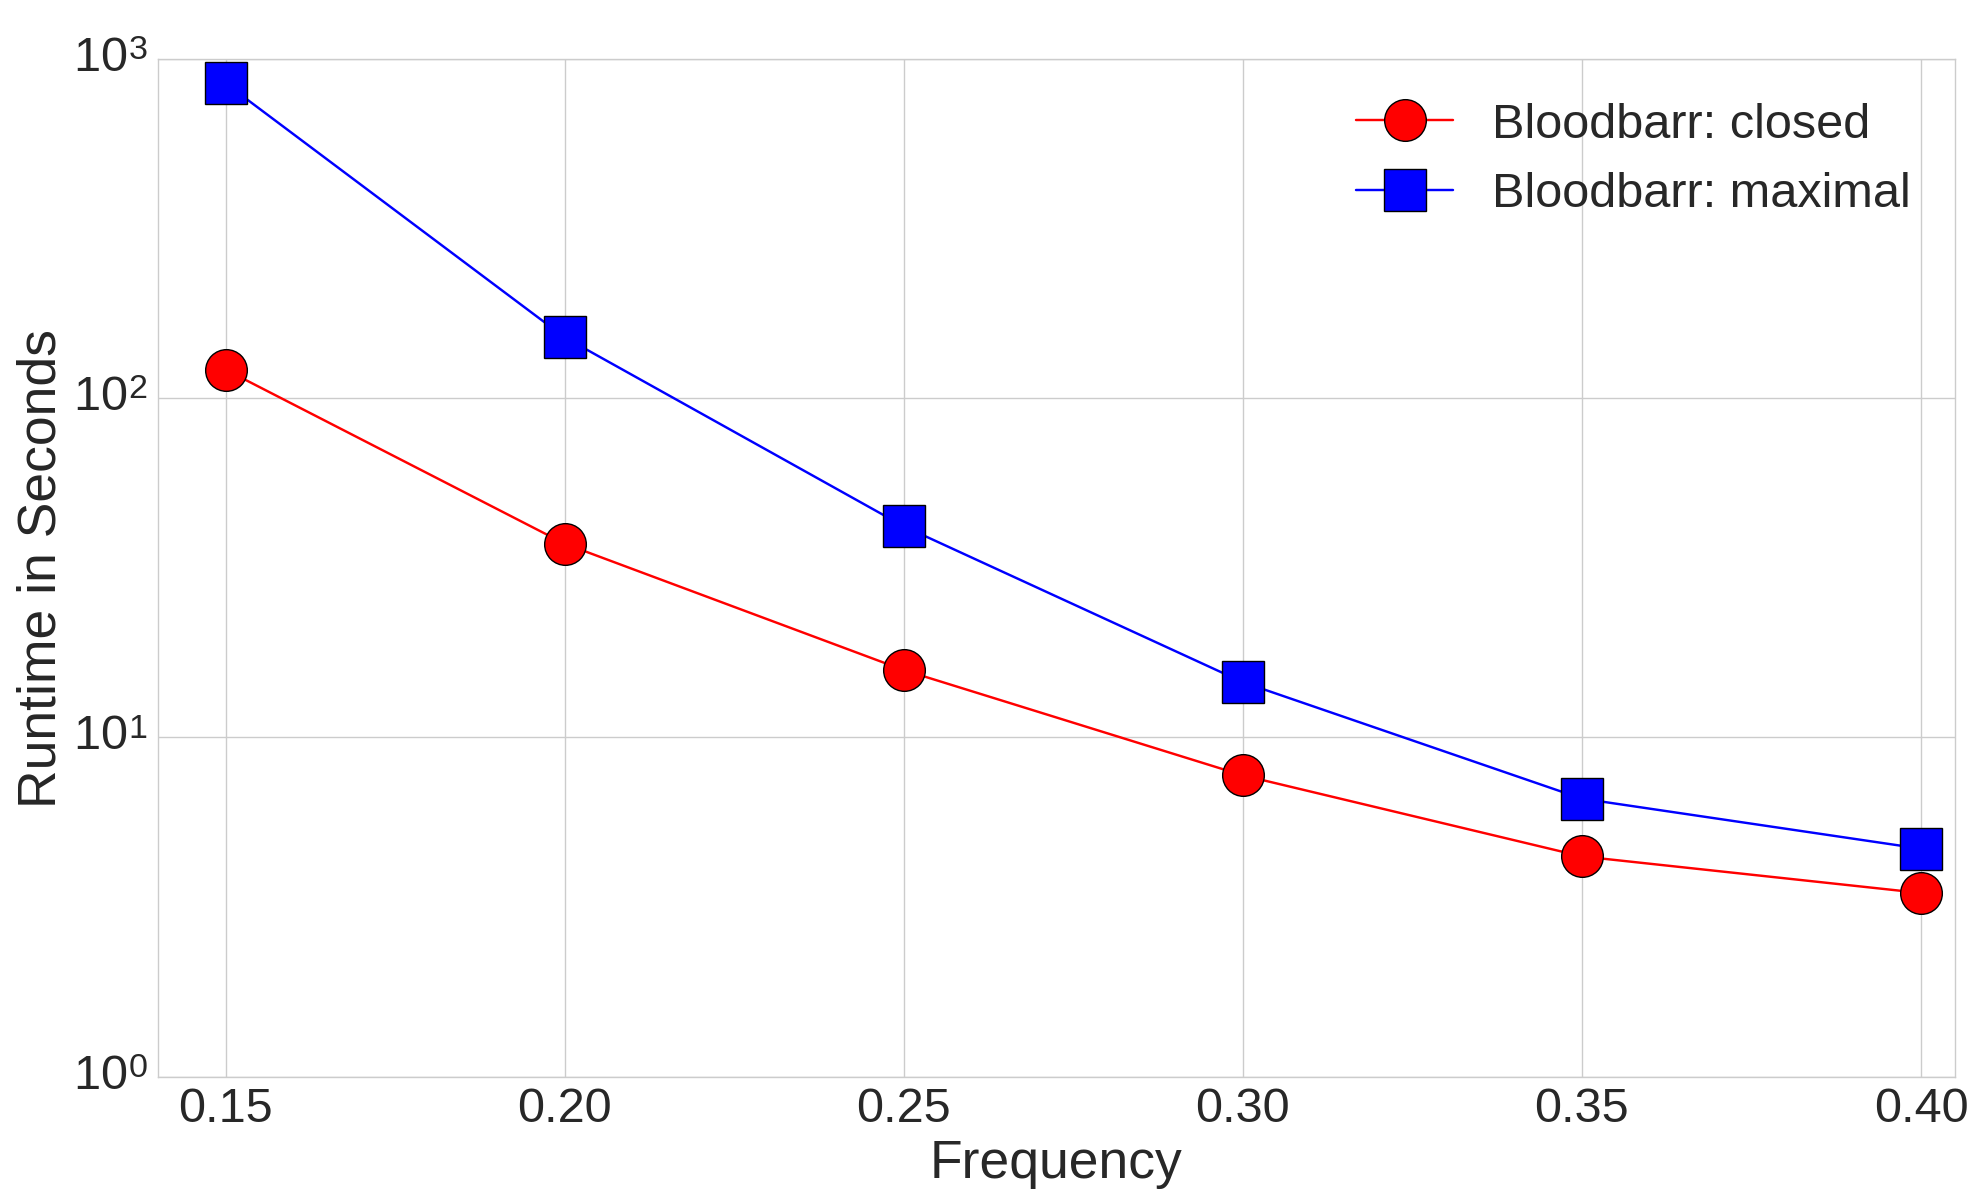
\includegraphics[width=\scalefigures\textwidth]{bloodbarr.png}
   \caption{Bloodbarr dataset: maximal and closed graph patterns}
    \label{fig:bloodbarr}
  \end{subfigure}
 \hfill
  \begin{subfigure}[t]{0.49\textwidth}
   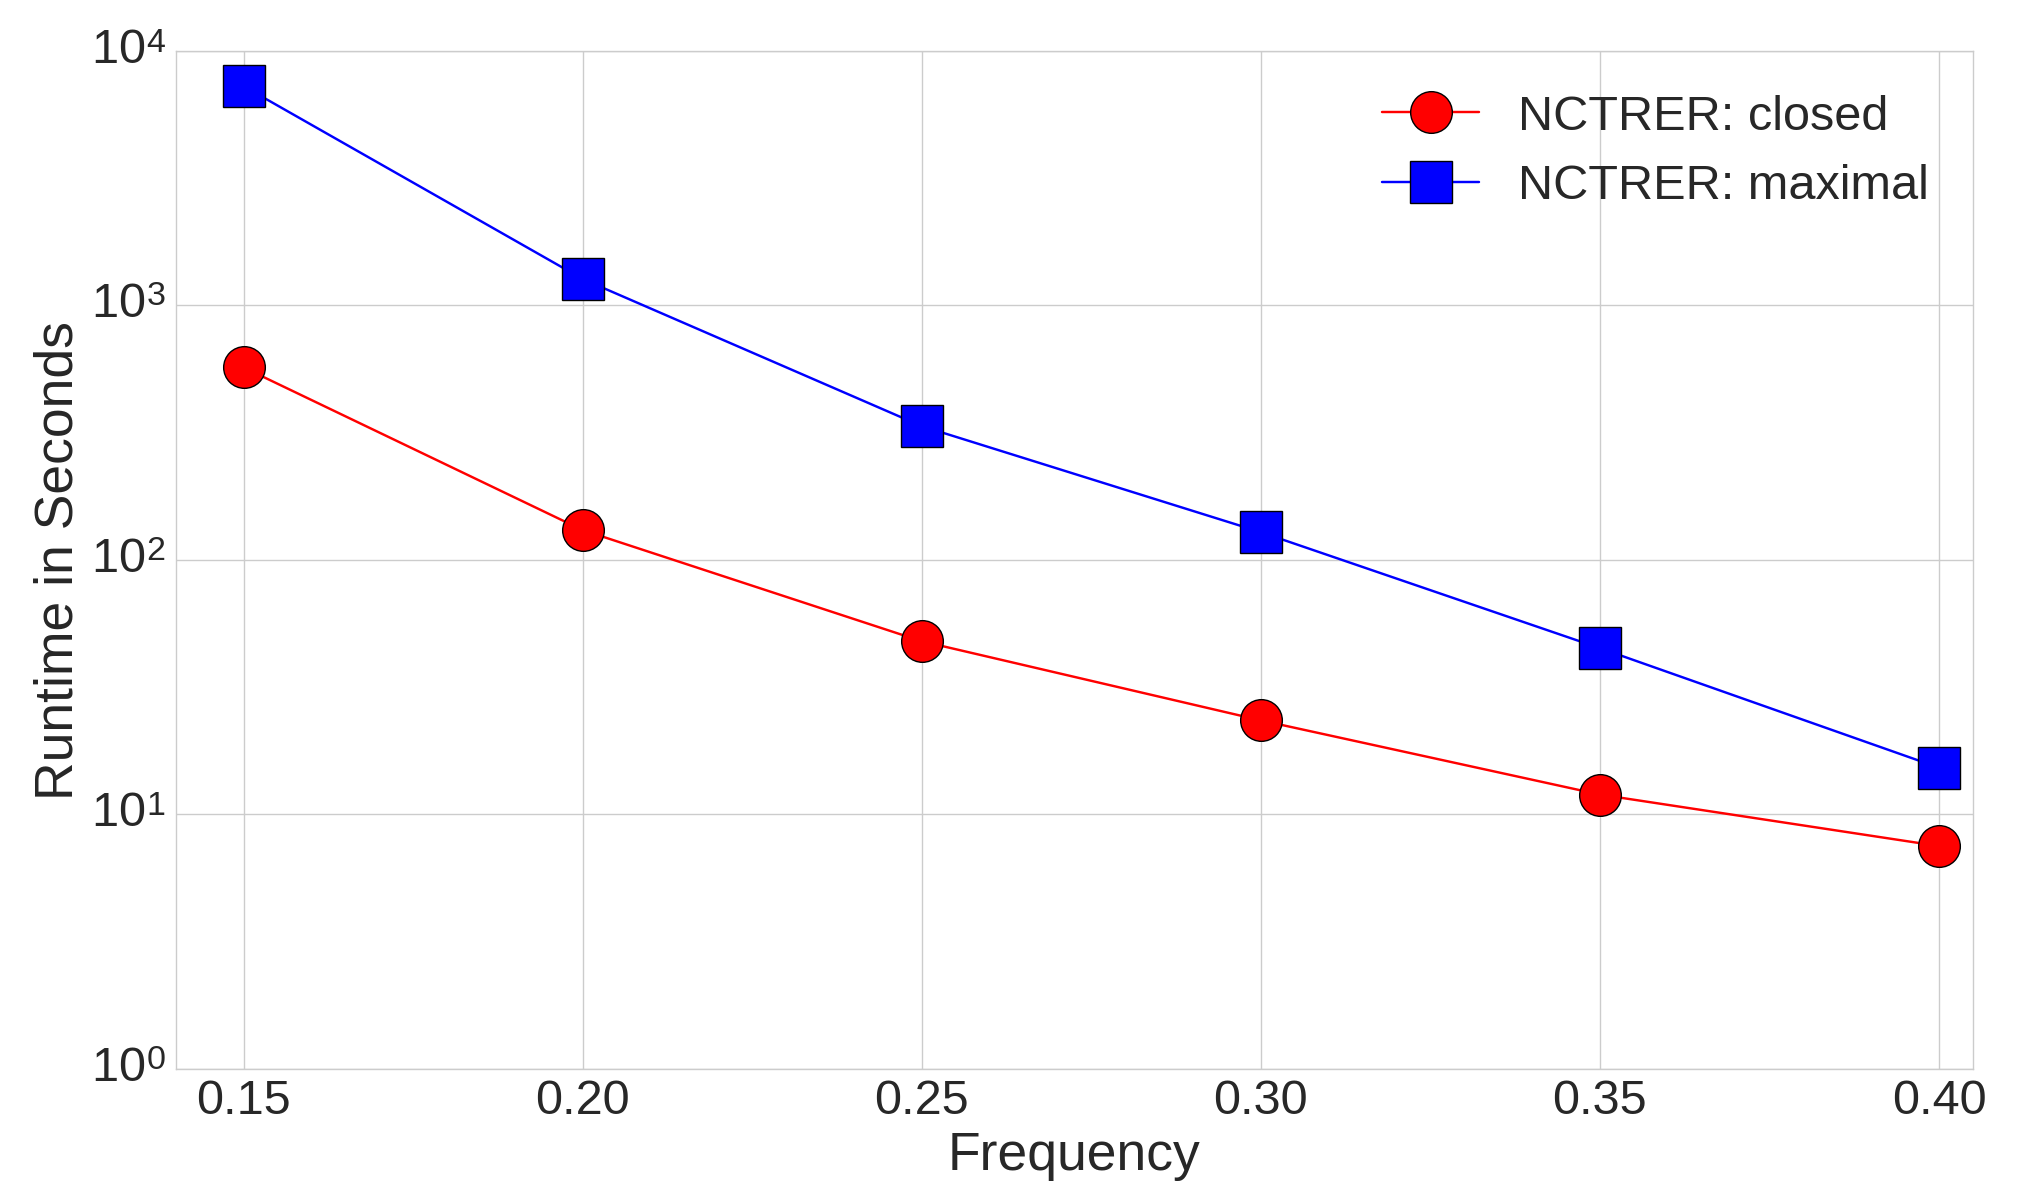
\includegraphics[width=\scalefigures\textwidth]{nctrer.png}
   \caption{Nctrer dataset: maximal and closed graph patterns}
    \label{fig:nctrer}
  \end{subfigure}
 \hfill
  \begin{subfigure}[t]{0.49\textwidth}
   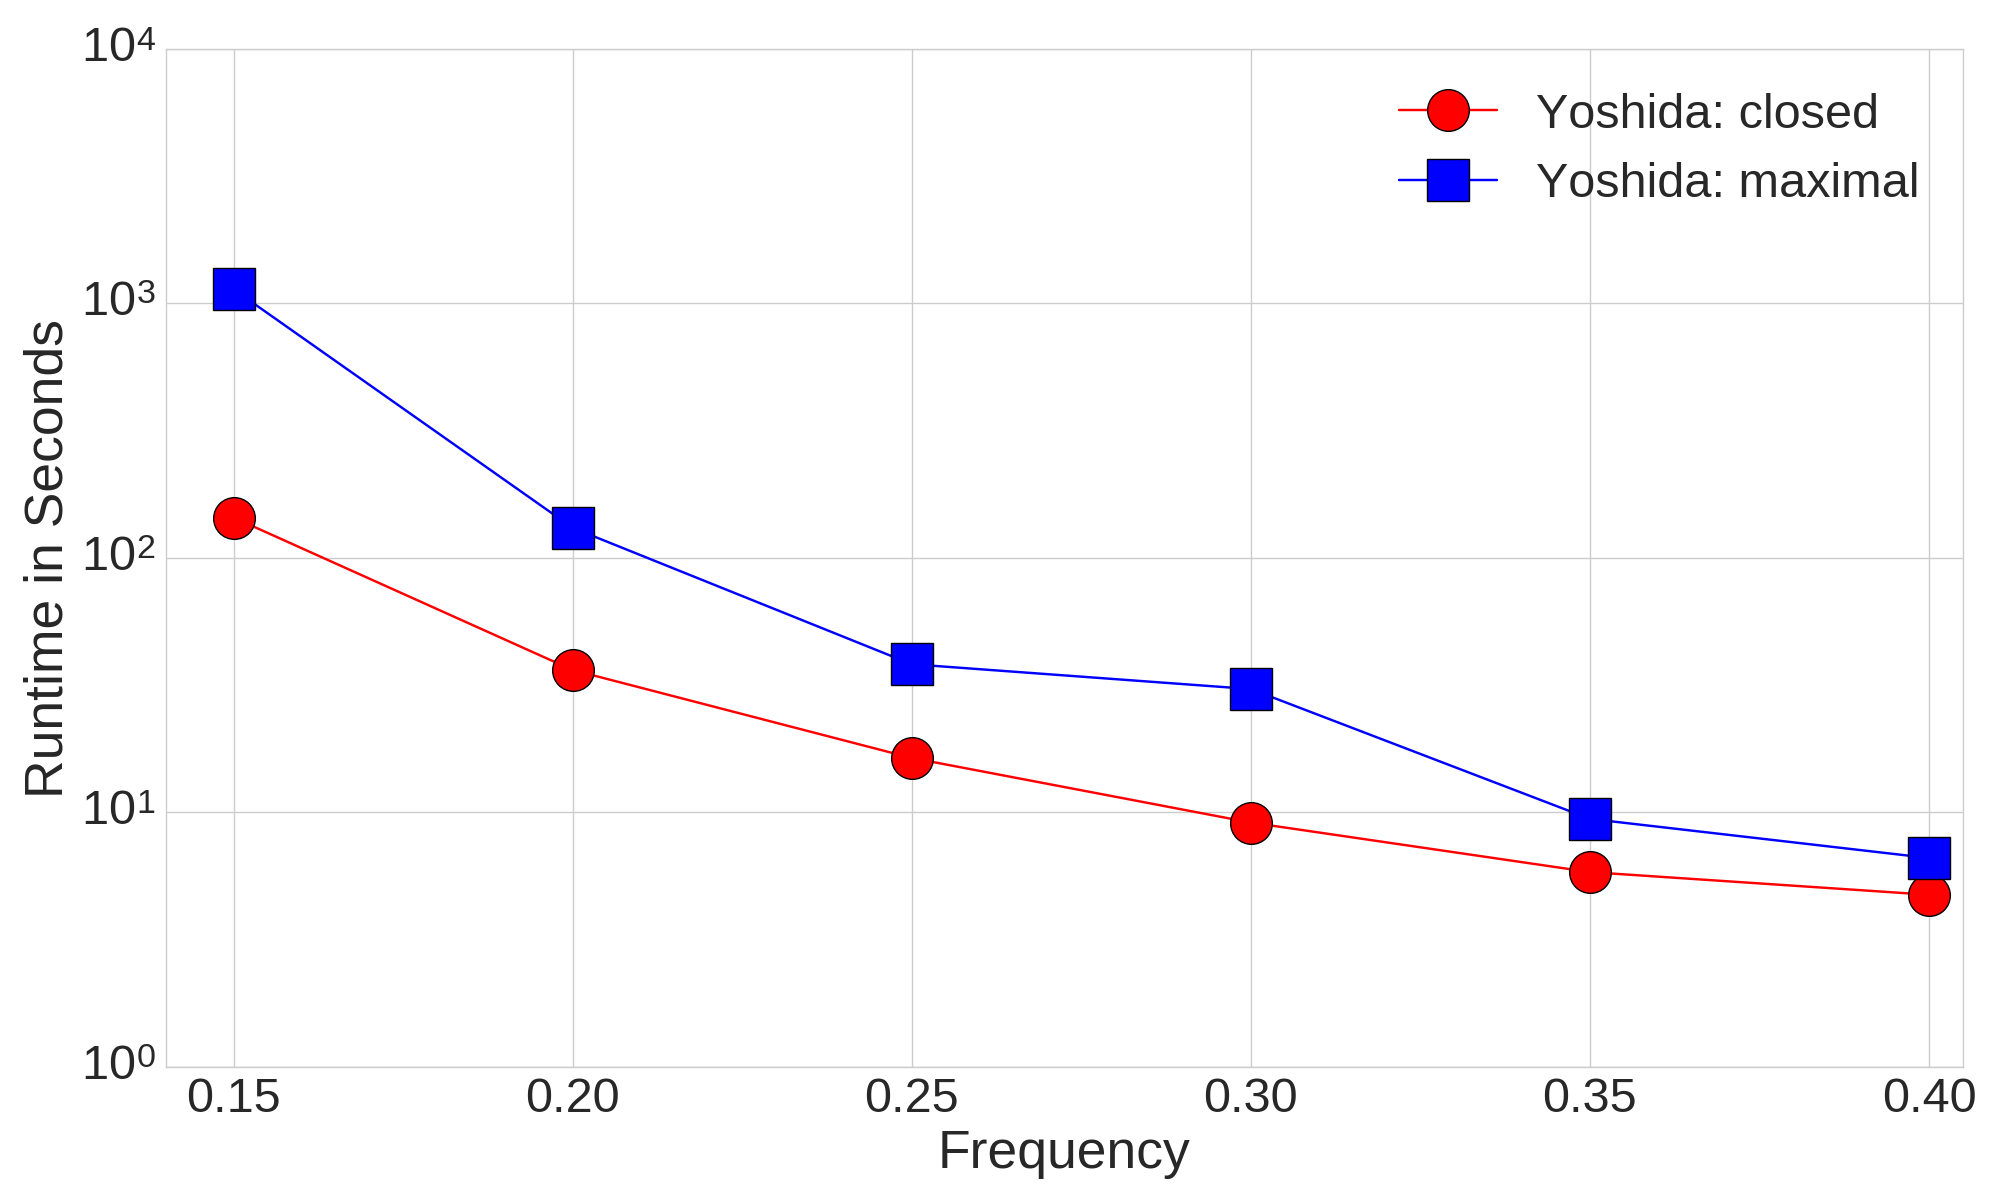
\includegraphics[width=\scalefigures\textwidth]{yoshida.png}
   \caption{Yoshida dataset: maximal and closed graph patterns}
    \label{fig:yoshida}
  \end{subfigure}
\hfill
  \begin{subfigure}[t]{0.49\textwidth}
   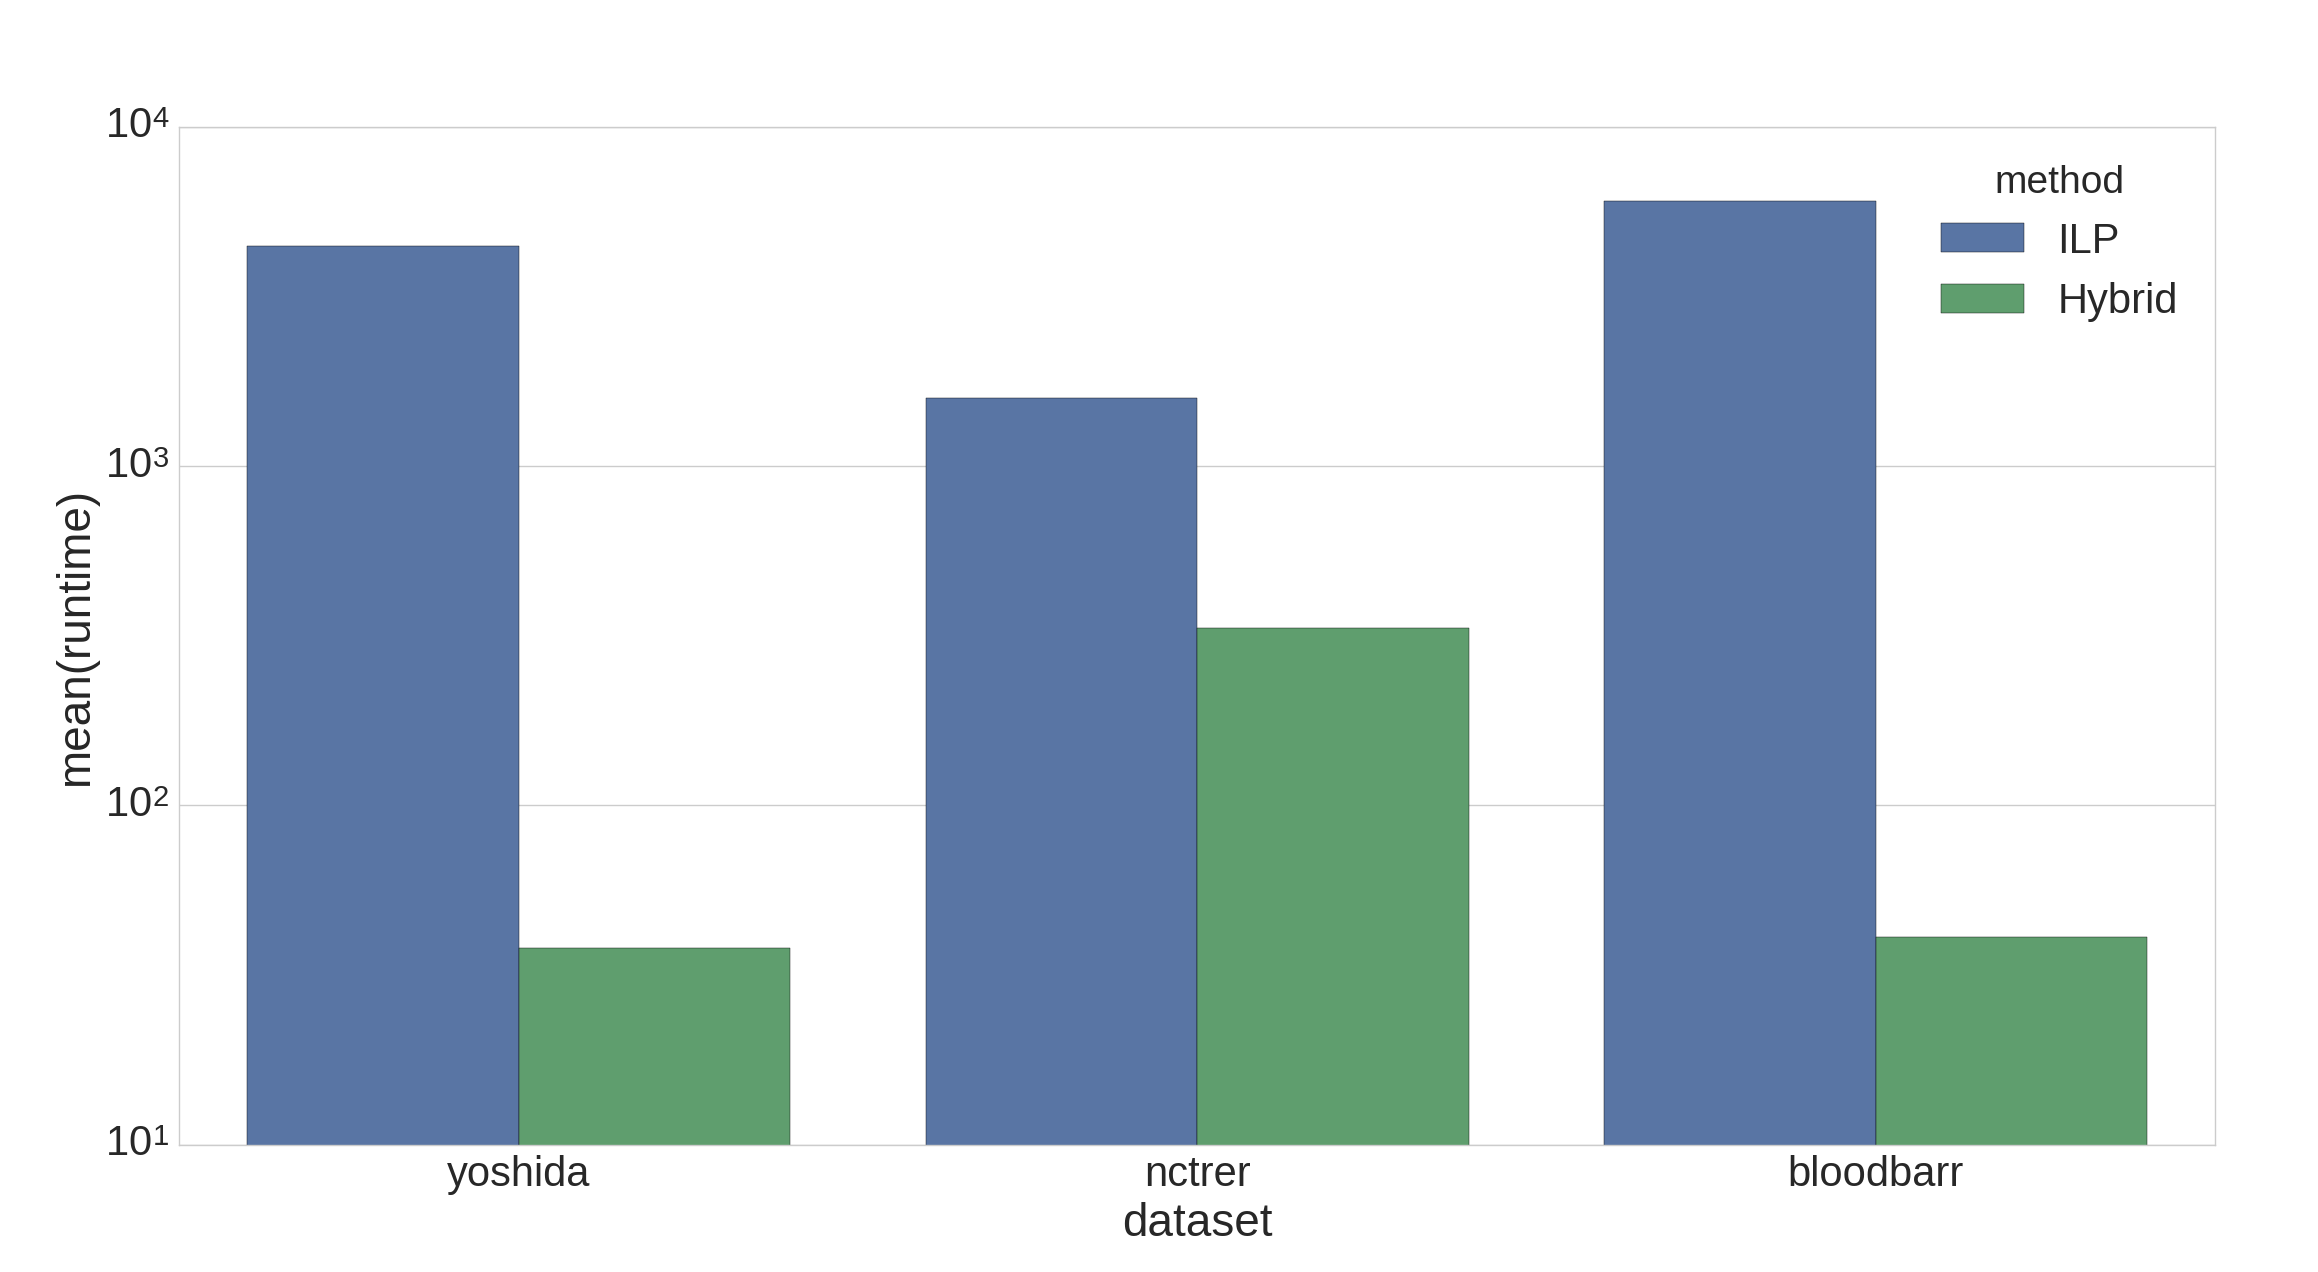
\includegraphics[width=\scalefigures\textwidth]{ILP_comparison.png}
   \caption{Comparison with logic programming ILP framework \parencite{query_mining_ilp}. For the ILP framework time to find \textit{a maximal solution} is indicated, while for our system  time to enumerate all maximal graph patterns (frequency $0.2$) is shown.}
   \label{fig:ilp_comparison}
  \end{subfigure}
  \label{fig:qfive}
  \caption{Investigating \qfive: evaluation on standard graph datasets (a,b,c) and comparison to the declarative ILP system for graph mining (d). Log-scale on all plots}
\end{figure}

To address \qfive, we consider the standard graph mining datasets 
in Figs. \ref{fig:bloodbarr}, \ref{fig:nctrer} and \ref{fig:yoshida}. One can observe, that our system is indeed able to handle real-sized datasets and process hundreds %and some 
or even thousands of graph patterns within the time-limit. Furthermore, the comparison with the purely declarative framework presented in Figure~\ref{fig:ilp_comparison} % we see that comparing with pure logic-programming framework, we 
demonstrates the two orders of magnitude speedup in runtime. In addition, note that our system is able to enumerate all condensed graph patterns, while the purely declarative approach is not capable of doing that within the timeout.
%\comment{Sergey: we need the description of Table \ref{til:div} here with a ref to \qsix}

To investigate \qsix, we tested our hybrid approach on the approximate tile selection problem from Def.~\ref{def:probtile}, exploiting Clasp reasoner for the ASP part of the algorithm. Since the considered problem is very computationally demanding, we did not set any timeout in this experimental setting. In Table~\ref{til:div} and Table~\ref{til:glass} we report the results for the Divorce and Glass datasets respectively. We compute the candidate tiles using an approach based on association confidences (see \textcite{dbp}). Given the set of candidate tiles, we use our ASP encoding from Listing~\ref{lst:tiles} to find all tilings whose overall error is below a specified threshold. We compare this approach to a greedy method for finding \emph{any} tiling that has error below the threshold. The greedy tiling approach\revision{, proposed by~\textcite{dbp},} will add the candidate tiles one-by-one until it has either found an admissible tiling, or it has exhausted all tiles. Note that, since the problem of finding the tiling is NP-hard, the greedy method is not guaranteed to find an admissible tiling even if one exists. 

The first column in Table~\ref{til:div} (respectively Table~\ref{til:glass}) reports the number $n$ of candidate tiles and the error threshold value $\sigma$. In the second column we present the details of the solution found by the \revision{greedy} method, i.e., the number $k$ of tiles in the solution tiling and its overall error. The computation of the tilings by the greedy algorithm takes less than a second. % \comment{DS: the time is pretty low, should we at all report it in the table? --- PM: We can drop it if we want; it's not very informative}
In the third column, the results of our hybrid approach are provided. More specifically, we present the number $k$ of tiles and the overall error for the first solution found by the solver together with the running time, as well as the details of the optimal tiling. To compute the optimal tiling we enforce the solver to find all models of the given ASP program (their total number is likewise reported). 

 The candidate tiles are computed by the dedicated algorithm within a fraction of a second, and the major computational efforts are done by the ASP solver to find the final tiling. Moreover, observe that since the grounding step is the most time-consuming, the time difference between the first found solution and all solutions including the optimal one is actually neglectable.
Note that comparing the running time of the \revision{greedy} and our hybrid algorithms is not entirely fair, as the former is not complete (i.e., it might not find any tiling, satisfying the conditions imposed by the error threshold even if one exists), which is in contrast to our hybrid approach.

The \revision{greedy} algorithm is capable of computing the optimal tiling only for small instances of the Divorce dataset. Starting from $n=5$, our hybrid method outperforms the \revision{greedy} one with respect to the quality of the found solutions. For the Glass dataset the benefit of our method is apparent even for smaller instances.

  

\leanparagraph{Summary} In all experiments, Step 1 of our method contributes to less than 5\% of runtime. %\comment{PM: Is this still true in the approximate case? -- DS: yes!} 
Overall, our approach can handle real world datasets for sequential pattern mining as demonstrated in \qone. In many cases %it 
its performance is %demonstrates performance 
close to the specialized mining languages, as % discussed 
shown in \qtwo. As demonstrated in \qthree various local constraints can be effectively incorporated into our encoding
bringing additional performance benefits. The choice of an ASP solver plays a crucial role in the overall performance of the system, as discussed in \qfour. In \qfive, it has been established that our approach leads to a significant speed up (of orders of magnitude) for the mining tasks with a complex structure, such as graph mining. Finally, the results of \qsix have proved the applicability of our hybrid framework for other computationally intensive data mining tasks, e.g., approximate tile selection problem, where our method is able to find solutions of higher quality.





% Please add the following required packages to your document preamble:
% \usepackage{multirow}
\begin{table}[]
\centering
\begin{tabular}{rrrrrrrrrr}
\hline
\multicolumn{1}{l}{\multirow{3}{*}{$n$/$\sigma$}} & \multicolumn{2}{c}{\revision{greedy}}                                                           & \multicolumn{7}{c}{hybrid}                                                                                                                                                                                                                                                              \\ \cline{2-10} 
\multicolumn{1}{l}{}                         & \multicolumn{1}{c}{\multirow{2}{*}{$k$}} & \multicolumn{1}{c}{\multirow{2}{*}{error}} & \multicolumn{3}{c}{first}                                                      & \multicolumn{1}{c}{\multirow{2}{*}{$k$ opt}} & \multicolumn{1}{c}{\multirow{2}{*}{error opt}} & \multicolumn{1}{c}{\multirow{2}{*}{time all}} & \multicolumn{1}{l}{\multirow{2}{*}{$|$all solutions$|$}} \\ \cline{4-6}
\multicolumn{1}{l}{}                         & \multicolumn{1}{c}{}                   & \multicolumn{1}{c}{}                       & \multicolumn{1}{l}{$k$} & \multicolumn{1}{l}{error} & \multicolumn{1}{l}{time} & \multicolumn{1}{c}{}                       & \multicolumn{1}{c}{}                           & \multicolumn{1}{c}{}                          & \multicolumn{1}{l}{}                                 \\ \hline
3/59                                           & 1                                       & 51                                          & 1                      & 59                         & 38.961                    & 1                                           & 51                                              & 38.962                                         & 5                                                     \\
4/54                                           & 1                                       & 51                                          & 2                      & 51                         & 38.127                    & 1                                           & 51                                              & 38.135                                         & 8                                                     \\
5/60                                           & 2                                       & 51                                          & 2                      & 58                         & 50.616                    & 2                                           & 47                                              & 50.617                                         & 15                                                    \\
6/60                                           & 2                                       & 51                                          & 2                      & 58                         & 50.601                    & 2                                           & 47                                              & 50.600                                         & 30                          \\ \hline                         
\end{tabular}
\caption{Addressing \qsix: approximate tiling problem  solution using specialized native algorithm for tile candidate generation and ASP encoding for selecting the resulting tiling (Divorce dataset)}
\label{til:div}
\end{table}


% Please add the following required packages to your document preamble:
% \usepackage{multirow}
\begin{table}[]
\centering
\begin{tabular}{rrrrrrrrrr}
\hline
\multicolumn{1}{c}{\multirow{3}{*}{$n$/$\sigma$}} & \multicolumn{2}{c}{\revision{greedy}}                                                           & \multicolumn{7}{c}{hybrid}                                                                                                                                                                                                                                                              \\ \cline{2-10} 
\multicolumn{1}{c}{}                         & \multicolumn{1}{c}{\multirow{2}{*}{$k$}} & \multicolumn{1}{c}{\multirow{2}{*}{error}} & \multicolumn{3}{c}{first}                                                      & \multicolumn{1}{c}{\multirow{2}{*}{$k$ opt}} & \multicolumn{1}{c}{\multirow{2}{*}{error opt}} & \multicolumn{1}{c}{\multirow{2}{*}{time all}} & \multicolumn{1}{c}{\multirow{2}{*}{$|$all solutions$|$}} \\ \cline{4-6}
\multicolumn{1}{c}{}                         & \multicolumn{1}{c}{}                   & \multicolumn{1}{c}{}                       & \multicolumn{1}{c}{$k$} & \multicolumn{1}{c}{error} & \multicolumn{1}{c}{time} & \multicolumn{1}{c}{}                       & \multicolumn{1}{c}{}                           & \multicolumn{1}{c}{}                          & \multicolumn{1}{c}{}                                 \\ \hline
3/214                                          & 1                                       & 184                                         & 1                      & 196                        & 294.172                   & 3                                           & 88                                              & 294.173                                        & 7                                                     \\
4/168                                          & 3                                       & 142                                         & 2                      & 154                        & 1194.088                  & 3                                           & 142                                             & 1194.093                                       & 2                                                     \\
5/222                                          & 3                                       & 180                                         & 3                      & 192                        & 2126.944                  & 4                                           & 142                                             & 2126.948                                       & 11                                                    \\
6/224                                          & 3                                       & 182                                         & 3                      & 194                        & 2198.739                  & 5                                           & 142                                             & 2198.743                                       & 25  \\ \hline                                                 
\end{tabular}
\caption{Addressing \qsix: approximate tiling problem solution using specialized native algorithm for tile candidate generation and ASP encoding for selecting the resulting tiling (Glass dataset)}
\label{til:glass}
\end{table}

%%% Local Variables:
%%% mode: latex
%%% TeX-master: "../aspmining_tplp.tex"
%%% End:
